\graphicspath{{4continuity/asy/}}

%\section{Continuity}
\setcounter{section}{16}


\section{Continuous Functions}\label{sec:cont}

For the rest of the course, we discuss continuous functions. Functions themselves should be familiar. For reference, we begin with a review of some basic concepts and conventions.\medbreak


We are concerned with functions $f:U\to V$ where both $U,V$ are subsets of the real numbers $\R$ and $f$ is some \emph{rule} assigning to each real number $x\in U$ a real number $f(x)\in V$. For instance
\[f(x)=\frac {x^2(x-7)}{(x-2)(x^2-9)} \quad\text{assigns to $x=1$ the value}\quad f(1)=\frac{1(-6)}{(-1)(-8)}=\frac 34\]
\begin{description}%\itemsep=3pt\parsep=3pt
	\item[\normalfont\emph{Domain}] $\dom f=U$ is the set of \emph{inputs} to $f$. When $f$ is defined by a formula, its \emph{implied domain} is the largest set on which the formula is defined: for the above example, $\dom f=\R\setminus\{2,3,-3\}$. In examples, the domain is typically a union of intervals of \emph{positive length.}
	\item[\normalfont\emph{Codomain}] $\operatorname{codom}f=V$ is the set of \emph{possible outputs.} In real analysis, we often take $V=\R$ by default.
	\item[\normalfont\emph{Range}] $\operatorname{range}f=f(U)=\{f(x):x\in U\}$; is the set of \emph{realized outputs.} It is a subset of $V$.
	\item[\normalfont\emph{Injectivity}] $f$ is \emph{injective/one-to-one} if distinct inputs produce distinct outputs. This is usually stated in the contrapositive: $f(x)=f(u)\implies x=u$.
	\item[\normalfont\emph{Surjectivity}] $f$ is \emph{surjective/onto} if every possible output is realized: otherwise said, $f(U)=V$.
	\item[\normalfont\emph{Inverses}] $f$ is \emph{bijective/invertible} if it is both injective and surjective. Equivalently, $f$ has an \emph{inverse function} $f^{-1}:V\to U$ defined as follows:
	\begin{itemize}
	  \item Given $y\in V$, $f$ surjective $\implies \exists x\in U$ such that $f(x)=y$.
	  \item Since $f$ is injective, $f(x)=f(u)\implies x=u$, so $x$ is unique. We \emph{define} $f^{-1}(y)=x$. 
	\end{itemize}
% 	The function $f^{-1}$ satisfies
% 	\[\forall u\in U,\ f^{-1}\bigl(f(u)\bigr)=u\quad\text{and}\quad \forall v\in V,\ f\bigl(f^{-1}(v)\bigr)=v\]
\end{description}

\begin{example}[lower separated=false, sidebyside, sidebyside align=top seam, sidebyside gap=0pt, righthand width=0.32\linewidth]{}{}
	The function defined by \smash{$f(x)=\frac 1{x(x-2)}$} has implied
	\begin{gather*}
		\textcolor{Green}{\dom f}=\R\setminus\{0,2\}=(-\infty,0)\cup(0,2)\cup (2,\infty)\\[5pt]
		\textcolor{Brown}{\operatorname{range} f}=(-\infty,-1]\cup(0,\infty)
	\end{gather*}
	The function is neither injective (e.g., $f(3)=f(-1)$) nor surjective (e.g., $0\not\in\operatorname{range}f$).\smallbreak
	We can remedy both issues by \textcolor{orange}{restricting} the domain and codomain. For instance, the same rule/formula but with
	\begin{gather*}
		\textcolor{Green}{\dom\hat f}=[1,2)\cup(2,\infty)\\
		\textcolor{Brown}{\operatorname{codom}\hat f}=(-\infty,-1]\cup(0,\infty)\\
		\intertext{defines a bijection with inverse function}
		\hat f^{-1}(y)=
		\begin{cases}
			1+y^{-1}\sqrt{y+1}&\text{if }y>0\\
			1-y^{-1}\sqrt{y+1}&\text{if }y\le -1
		\end{cases}
	\end{gather*}
	Observe that $\textcolor{Brown}{\dom\hat f^{-1}}=\textcolor{Green}{\operatorname{codom}\hat f}$ and $\textcolor{Green}{\operatorname{codom}\hat f^{-1}}=\textcolor{Brown}{\dom\hat f}$.
	\tcblower
	\flushright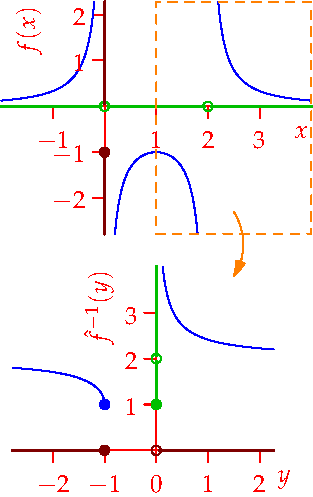
\includegraphics{dom4}
\end{example}

\goodbreak


To introduce continuity, we consider two common naïve notions.
\begin{description}
  \item[The graph of $f$ can be drawn without removing one's pen from the page] This is intuitive but unusable: \emph{drawn} is poorly defined, so how could we \emph{calculate} or \emph{prove} anything with this concept? Moreover, it cannot reasonably be extended to other situations (e.g.,\ multivariable functions) where drawing a graph is meaningless.
  \item[If $x$ is close to $a$, then $f(x)$ is close to $f(a)$] This is better and can be generalized to other situations. The major issue is the unclear meaning of \emph{close.} Our formal definition of continuity addresses this using \emph{sequences} and \emph{limits.}
\end{description}


\begin{defn}{Sequential continuity}{seqcont}
	Let $f:U\to V\subseteq\R$ be a function. We say that \emph{$f$ is continuous at $u\in U$} if,
	\[\forall (x_n)\subseteq U,\text{ we have }\lim x_n=a\implies\lim f(x_n)=f(a)\]
	$f$ is \emph{continuous (on $U$)} if it is continuous at every point $a\in U$.\smallbreak
	A \emph{discontinuity} of $f$ is a value $a\in U$ at which $f$ is \emph{discontinuous} (not continuous),
	\[\exists (x_n)\subseteq U,\text{ such that }\lim x_n=a\text{ and }\bigl(f(x_n)\bigr)\text{ does not converge to $f(a)$}\]
	\begin{minipage}[t]{0.49\linewidth}\vspace{0pt}
		\centering
		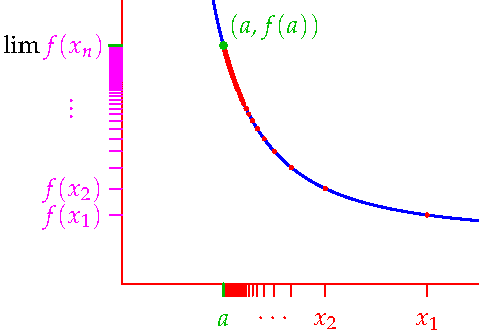
\includegraphics{contdef-pic4}\\
		Continuity at $\textcolor{Green}{a}$: \emph{every sequence}\par
		with $\lim\textcolor{red}{x_n}=\textcolor{Green}{a}$ has $\lim\textcolor{magenta}{f(x_n)}=\textcolor{Green}{f(a)}$
	\end{minipage}
	\hfill
	\begin{minipage}[t]{0.49\linewidth}\vspace{0pt}
		\centering
		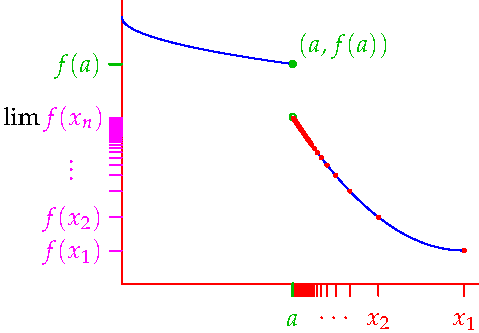
\includegraphics{contdef-pic2}\\
		Discontinuity at $\textcolor{Green}{a}$: \emph{at least one sequence}\\
		with $\lim\textcolor{red}{x_n}=\textcolor{Green}{a}$ has $\lim\textcolor{magenta}{f(x_n)}\neq \textcolor{Green}{f(a)}$
	\end{minipage}
\end{defn}


\begin{examples}{}{basiccont}
	\exstart $f:\R\to\R:x\mapsto x^2$ is continuous (at every $a\in\R$). To see this, suppose $(x_n)$ converges to $a$, then, by the limit laws,
  \[\lim f(x_n)=\lim x_n^2=(\lim x_n)^2=a^2=f(a)\]
  
  \begin{enumerate}\setcounter{enumi}{1}
	  \item The function with $g(x)=1+\frac 4{x^2}$ is continuous. Choose any $a\in\dom g=\R\setminus\{0\}$ and any $(x_n)\subseteq\dom g$ with $\lim x_n=a$. Again, by the limit laws,
	  \[\lim g(x_n)=\lim\left(1+\frac 4{x_n^2}\right) =1+\frac 4{(\lim x_n)^2}=1+\frac 4{a^2}=f(a)\]
	  This example (with $a=1$ and $x_n=1+\frac 2n$) is the first picture in the definition.
  
  \item $h:[0,\infty)\to\R:x\mapsto 3x^{1/4}$ is continuous. Again, everything follows from the limit laws. If $x_n\to a$ where $x_n\ge 0$ and $a\ge 0$, then
  \[\lim h(x_n)=\lim 3x_n^{1/4}=3(\lim x_n)^{1/4}=3a^{1/4}=h(a)\]
  
	\begin{minipage}[t]{0.70\linewidth}\vspace{-5pt}
  	\item The function defined by
	  \[
	  	k(x)=
	  	\begin{cases}
	  		1+2x^2&\text{if }x<1\\
	  		2-x&\text{if }x\ge 1
	  	\end{cases}
	  \]
  	is discontinuous at $a=1$. This seems obvious from the picture, but we need to use the definition. The sequence with $x_n=1-\frac 1n$ converges to 1 from below, whence
  	\[\lim k(x_n)=\lim \left(1+2\left(1-\frac 2n+\frac 1{n^2}\right)\right)=3\neq 1=k(1)\]
	\end{minipage}
	\hfill
	\begin{minipage}[t]{0.29\linewidth}\vspace{-5pt}
		\flushright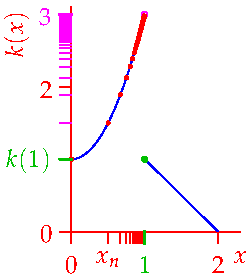
\includegraphics{cont-ex2}
	\end{minipage}


  
%   \item The function with $f(x)=\begin{cases}
%   8-\sqrt x&\text{ if }0\le x\le 2\\
%   1+(x-4)^2&\text{ if }x>2
%   \end{cases}$\quad is continuous except at $x=2$.
%   \begin{itemize}
%     \item Suppose $a>2$ and let $x_n\to a$. Then
%     \[\exists N\text{ such that }n>N\implies x_n>2\implies f(x_n)=1+(x_n-4)^2\]
%     By the limit laws, we have $\lim f(x_n)=1+(a-4)^2=f(a)$, whence $f$ continuous at $x=a$.
%     \item The case where $a<2$ is similar: let $x_n\to a$, then
%     \[\exists N\text{ such that }n>N\implies x_n<2\implies f(x_n)=8-\sqrt{x_n}\]
%     By the limit laws, we clearly have $\lim f(x_n)=8-\sqrt{a}=f(a)$.
%     \item If $a=2$, consider the sequence with $x_n=2+\frac 1n$. Then $x_n\to a$, but
%     \[x_n>2\implies f(x_n)=1+(x_n-4)^2\to 1\neq 8-\sqrt 2=f(a)\]
%     We conclude that $f$ is not continuous at $x=2$. This case is drawn in the second picture shown previously.
%   \end{itemize}
\end{enumerate}
\end{examples}

\boldsubsubsection{Basic examples and combinations of continuous functions}

By appealing to the limit laws for sequences (Theorem \ref{thm:limitbasic}), we can combine continuous functions in natural ways. For instance, if $f,g$ are continuous at $a$, then
\[\lim x_n=a\implies \lim f(x_n)+g(x_n)=\lim f(x_n)+\lim g(x_n)=f(a)+g(a)\]
whence $f+g$ is continuous at $a$. Here is a general summary.

\begin{thm}{}{contsimple}
\exstart Suppose $f,g$ are continuous and that $k$ is constant. Then the following functions are continuous (on their domains)
	\[kf,\quad \nm f,\quad f+g,\quad f-g,\quad fg,\quad \frac fg,\quad \max(f,g),\quad \min(f,g)\]
\begin{enumerate}\setcounter{enumi}{1}
	\item If $n\in\N$ then the function $f:x\mapsto x^{1/n}$ is continuous on its domain.
	\item Compositions of continuous functions are continuous. Specifically, if $g$ is continuous at $a$ and $f$ is continuous at $g(a)$, then $f\circ g$ is continuous at $a$.
	\item Algebraic functions are continuous (this includes all polynomials and rational functions).
\end{enumerate}
\end{thm}

\begin{proof}
Parts 1, 2 are the limit laws; for the maximum and minimum, see Exercise \ref{exs:maxcont}. For part 3:
\[\lim x_n=a\overset{g\text{ cont}}\implies \lim g(x_n)=g(a) 
\overset{f\text{ cont}}\implies \lim f\bigl(g(x_n)\bigr)=f\bigl(g(a)\bigr)\]
Part 4 follows from parts 1, 2 and 3. 
\end{proof}


\begin{example}{}{}
Part 3 of the theorem says that the following algebraic function is continuous
\[f:(7,\infty)\to\R:x\mapsto \sqrt{\frac{3x^{5/2}+7x^2+4}{(x-7)^{1/3}}}\]
\end{example}

\goodbreak


\begin{thm}{Squeeze theorem}{}
Suppose $f(x)\le g(x)\le h(x)$ for all $x\neq a$, that $f,h$ are continuous at $a$, and that $f(a)=g(a)=h(a)$. Then $g$ is continuous at $a$. 
\end{thm}

\begin{proof}
This is simply the squeeze theorem (\ref{thm:squeeze}) for sequences: if $\lim x_n=a$, then
\[f(x_n)\le g(x_n)\le h(x_n)\implies \lim g(x_n)=g(a)\tag*{\qedhere}\]
\end{proof}

To provide more interesting examples, we state the following without proof.

\begin{thm}{}{conttrig}
The common trigonometric, exponential and logarithmic functions are continuous.
\end{thm}

It is possible, though slow and ugly to address some of this now, though it is not very profitable. It is better to define these functions later using power series\footnote{For instance via the Maclaurin series $e^x=\sum\limits_{n=0}^\infty\frac{x^n}{n!}$, $\sin x=\sum\limits_{n=0}^\infty\frac{(-1)^n}{(2n+1)!}x^{2n+1}$ and $\cos x=\sum\limits_{n=0}^\infty\frac{(-1)^n}{(2n)!}x^{2n}$} when their continuity (and differentiability/integrability!) come for free.

\begin{examples}{}{}
\exstart $f(x)=\frac{\sqrt x}{\sin e^x}$ is continuous on its domain $\R\setminus\{\ln(n\pi):n\in\N_0\}$.
\begin{enumerate}\setcounter{enumi}{1}
	\begin{minipage}[t]{0.70\linewidth}\vspace{-5pt}
		\item The function defined by $g(x)=x\sin\frac 1x$ if $x\neq 0$ and $g(0)=0$ is continuous on $\R$. When $x\neq 0$, this follows from Theorems \ref{thm:contsimple} and \ref{thm:conttrig}, while at $a=0$ we rely on the squeeze theorem:
		\[x\neq 0\implies -x\le x\sin\frac 1x\le x\]
	\end{minipage}
	\hfill
	\begin{minipage}[t]{0.29\linewidth}\vspace{-5pt}
		\flushright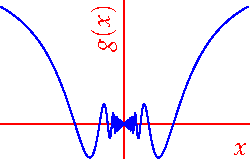
\includegraphics{cont-ex1}
	\end{minipage}
\end{enumerate}
\end{examples}


\boldsubsubsection{The $\epsilon$--$\delta$ Definition of Continuity}\phantomsection\label{ex:easycont2}

The sequential definition of continuity uses limits \emph{twice.} By stating each of these using the $\epsilon$-definition of limit, we can reformulate continuity without ever mentioning sequences.\smallbreak

To motivate this, consider $f(x)=x^2$ at $a=2$. By continuity, if $(x_n)$ is a sequence with $\lim x_n=2$, then $\lim f(x_n)=4$. We restate each of these using the definition of limit:
	\begin{itemize}
	  \item[(a)] ($\lim x_n=2$)\quad $\forall\delta>0$, $\exists M$ such that $n>M\implies \nm{x_n-2}<\delta$
	  \item[(b)] ($\lim x_n^2=4$)\quad $\forall\epsilon>0$, $\exists N$ such that $n>N\implies \nm{x_n^2-4}<\epsilon$
	\end{itemize}
	Here is a short argument that shows how (a)\,$\Rightarrow$\,(b) (we'll revisit this formally in a moment).\medbreak
	 
	Assume (a), let $\epsilon>0$ be given, and \emph{define} $\delta=\min(1,\frac\epsilon 5)$. Since $\lim x_n=2$, $\exists M$ such that
	\begin{align*}
	n>M \implies  \nm{x_n^2-4}&=\nm{x_n-2}\nm{x_n+2} <\delta\nm{(x_n-2)+4} \tag{by (a)}\\
	&\le \delta\bigl(\nm{x_n-2}+4\bigr)\tag{$\triangle$-inequality}\\
	&<\delta(\delta+4)\le 5\delta\le\epsilon \tag{(a) again}
	\end{align*}
	Let $N=M$ to conclude (b).\medbreak
	It turns out not to be very important that $(x_n)$ be a \emph{sequence.} In fact we can dispense with it entirely\ldots
%\end{example*}

\goodbreak


\begin{defn}{$\epsilon$--$\delta$ continuity}{epcont}
	A function $f:U\to V\subseteq\R$ is continuous at $a$ if\footnotemark{}
	\[\forall\epsilon>0,\ \exists\delta>0\text{ such that }(\forall x\in U)\ \nm{x-a}<\delta\implies\nm{f(x)-f(a)}<\epsilon\tag{$\ast$}\]
	A \emph{discontinuity} of $f$ is a value $a\in U$ for which,
	\[\exists\epsilon>0\ \text{such that}\ \forall\delta>0,\ \exists x\in U\ \text{with }\nm{x-a}<\delta\ \text{and}\ \nm{f(x)-f(a)}\ge\epsilon\tag{$\dag$}\]
	
	\begin{minipage}[t]{0.49\linewidth}\vspace{-12pt}
		\centering
		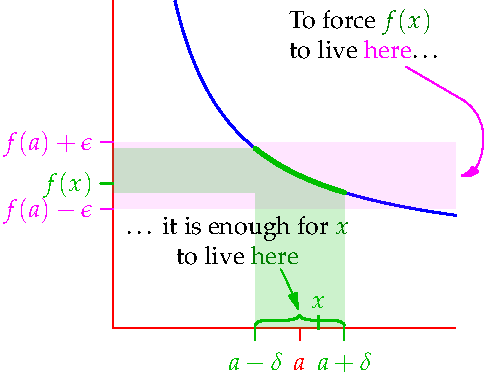
\includegraphics[scale=0.95]{contdef-pic5}\\
		Continuity at $a$
	\end{minipage}
	\hfill
	\begin{minipage}[t]{0.49\linewidth}\vspace{-12pt}
		\centering
		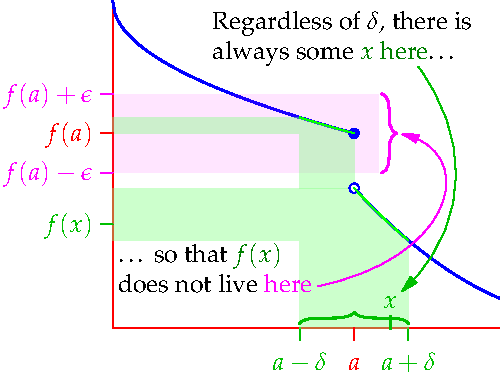
\includegraphics[scale=0.95]{contdef-pic3}\\
		Discontinuity at $a$
	\end{minipage}
\end{defn}

\footnotetext{The bracketed statement $\forall x\in U$ is often omitted in ($\ast$), since the implication requires $x$ to be universally quantified. It is important that $x\in U=\dom f$ rather than merely $x\in\R$! By contrast, the expression $\exists x\in U$ in ($\dag$) is \emph{always} written.}

This is the intuitive interpretation of continuity: if $x$ is close to $a$, then $f(x)$ is close to $f(a)$; $\epsilon$ and $\delta$ are merely measures of closeness. Most mathematicians consider the $\epsilon$--$\delta$ version to be \emph{the} definition of continuity. Thankfully, it doesn't matter which you prefer\ldots

\begin{thm}{}{cont}
	The sequential and $\epsilon$--$\delta$ definitions of continuity (\ref{defn:seqcont} \& \ref{defn:epcont}) are equivalent.
\end{thm}


\begin{examples*}{\ref{ex:basiccont}, cont}{}
	Before seeing the proof, we repeat our earlier examples using the $\epsilon$--$\delta$ definition. As with $\epsilon$--$N$ arguments for limits, it is often useful to do some scratch work first.

	\begin{enumerate}
  	\item Suppose $f(x)= x^2$ and $a\in\R$. Our goal is to control the size of $\nm{x^2-a^2}$ whenever $\nm{x-a}$ is small. To keep things simple, assume $\nm{x-a}<1$, then,
  	\begin{align*}
  		\nm{x^2-a^2}&=\nm{x-a}\nm{x+a}=\nm{x-a}\bigl|(x-a)+2a\bigr|\\
  		&\overset{\triangle}{\le}\nm{x-a}\bigl(\nm{x-a}+2\nm a\bigr) =\nm{x-a}(1+2\nm a)
  	\end{align*}
 		Now let $\epsilon>0$ be given and define $\delta=\min(1,\frac\epsilon{1+2\nm a})$. Then
  	\begin{align*}
	  	\nm{x-a}<\delta\implies\nm{f(x)-f(a)}&=\nm{x^2-a^2} <\delta(1+2\nm a)\le\epsilon
  	\end{align*}
  	Thus $f$ is continuous at $a$. This is simply a general version of the argument on page \pageref{ex:easycont2} with all mention of sequences removed!
  
  	\goodbreak
  
 
  	\item Let $g(x)= 1+\frac 4{x^2}$ and $a\neq 0$. The first challenge is to control $\frac 1x$ by staying away from zero: to do this, we start by insisting that $\delta\le\frac{\nm a}2$. But now,
  	\[
  		\nm{x-a}<\delta\implies \nm x>\frac{\nm a}2 \implies \frac 1{\nm x}<\frac 2{\nm a}\tag{$\ast$}
  	\]
  	Now consider the required difference; if $\nm{x-a}<\delta$, then
	  \begin{align*}
			\nm{g(x)-g(a)} &=\nm{1+\frac 4{x^2}-1-\frac 4{a^2}}=\frac{4\nm{a^2-x^2}}{a^2x^2}=\frac{4\nm{a+x}}{a^2x^2}\nm{x-a}\\
	  &\overset{\triangle}{\le} 4\left(\frac 1{\nm ax^2}+\frac 1{a^2\nm x}\right)\nm{x-a} \overset{(\ast)}{<} 4\left(\frac 4{\nm a^3}+\frac 2{\nm a^3}\right)\nm{x-a} = \frac{24}{\nm{a}^3}\delta
  	\end{align*}
 		Given $\epsilon>0$, it suffices to let $\delta=\min(\frac 12\nm a,\frac 1{24}{\nm a^3}\epsilon)$. Then $\nm{x-a}<\delta\implies \nm{f(x)-f(a)} <\epsilon$.
  	%We conclude that $g$ is continuous on $\R\setminus\{0\}$.
  
	  \item For $h(x)=3x^{1/4}$, there are two cases. Suppose $\epsilon>0$ is given.
	  \begin{itemize}
	    \item If $a=0$, let $\delta=\left(\frac\epsilon 3\right)^4$, then\footnotemark{}
	  	\begin{align*}
	  		\nm{x-a}<\delta\implies 0\le x<\delta\implies \nm{h(x)-h(a)}=3x^{1/4}<3\delta^{1/4}=\epsilon
	  	\end{align*}
	    \item If $a>0$, let $\delta=\frac 13a^{3/4}\epsilon$. Then, if $\nm{x-a}<\delta$, we have
	    \[
	    	\nm{h(x)-h(a)}=3\nm{x^{1/4}-a^{1/4}}=\frac{3\nm{x-a}}{x^{\frac 34}+a^{\frac 14}x^{\frac 24}+a^{\frac 24}x^{\frac 14}+a^{\frac 34}} \le\frac{3\nm{x-a}}{a^{3/4}}<\frac{3\delta}{a^{3/4}} =\epsilon
	    \]
	  \end{itemize}
    
  	\begin{minipage}[t]{0.7\linewidth}\vspace{0pt}
	  	\item Suppose $k$ is continuous at 1 and let $\epsilon=1$. Then $\exists \delta>0$ for which
	  	\begin{align*}
			  \nm{x-1}<\delta&\implies \nm{k(x)-k(1)}=\nm{k(x)-1}<1\\
			  &\implies \textcolor{magenta}{0<k(x)<2}
		  \end{align*}
	  	However, if we choose $x=\max(\frac 1{\sqrt 2},1-\frac\delta 2)$, then $\textcolor{Green}{\nm{x-1}\le \frac\delta 2<\delta}$ and $k(x)\ge k(\frac 1{\sqrt 2})=1+\frac 22=2$. Contradiction.
	  \end{minipage}
	  \hfill
	  \begin{minipage}[t]{0.27\linewidth}\vspace{-2pt}
	  	\flushright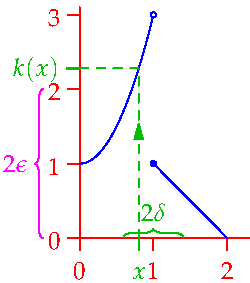
\includegraphics[scale=0.9]{cont-ex3}
	  \end{minipage}
	  
  \end{enumerate}
  
\end{examples*}

\footnotetext{Remember the hidden quantifier: $\nm{x-a}<\delta$ \emph{for all} $x\in\dom f=[0,\infty)$, thus $x\ge 0$ for the duration of this example.}

The basic rules for combining continuous functions may also be proved using $\epsilon$--$\delta$ arguments. E.g.,

\begin{proof}[$\epsilon$--$\delta$ proof of the squeeze theorem]
Given $\epsilon>0$, we know there exist $\delta_1,\delta_2>0$ for which
	\[
		\nm{x-a}<\delta_1\implies \nm{f(x)-f(a)}<\epsilon\quad\text{and}\quad
		\nm{x-a}<\delta_2\implies \nm{h(x)-h(a)}<\epsilon
	\]
	Let $\delta=\min(\delta_1,\delta_2)$, then
  \[
  	\nm{x-a}<\delta\implies\nm{g(x)-g(a)}\le\max\bigl(\nm{f(x)-f(a)},\nm{h(x)-h(a)}\bigr) <\epsilon
  \]
	whence $g$ is continuous at 0.
\end{proof}

Several other arguments are in the exercises. Finally, here is the promise proof of equivalence.



% 
% Since the $\epsilon$--$\delta$ approach is so much trickier, it is reasonable to ask why anyone would choose it over the sequential. Here are a few answers:
% \begin{enumerate}
%   \item The $\epsilon$-approach generalizes to higher dimensions with little increase in difficulty.
%   \item Sequences require more, and uglier, notation/subscripts which can get in the way when examples are more complicated.
%   \item Critical upcoming concepts such as \emph{uniform continuity} (section \ref{sec:uniformcont}) need the $\epsilon$-approach.
% \end{enumerate}

\goodbreak


\begin{proof}[Proof of Theorem \ref{thm:cont}]
\begin{description}
\item[\normalfont(sequential $\Rightarrow\epsilon$--$\delta$)] We prove the contrapositive. Suppose $a$ is an $\epsilon$--$\delta$ discontinuity ($\dag$) and let $\delta=\frac 1n$. Then there exists $x_n\in U$ such that
	\[\nm{x_n-a}<\frac 1n\quad\text{and}\quad \nm{f(x_n)-f(a)}\ge\epsilon\]
	Repeating for all $n\in\N$ results in a sequence $(x_n)$ for which $\lim x_n=a$ and $\lim f(x_n)\neq f(a)$: otherwise said, $a$ is a sequential discontinuity.
	
	\item[\normalfont($\epsilon$--$\delta\Rightarrow$ sequential)] Assume ($\ast$), let $(x_n)\subseteq U$ and suppose $\lim x_n=a$; we must prove that $\lim f(x_n)=f(a)$. Let $\epsilon>0$ be given so that a suitable $\delta$ satisfying ($\ast$) exists. Since $\lim x_n=a$,
	\begin{align*}
		\exists N\text{ such that }n>N&\implies \nm{x_n-a}<\delta\tag{since $x_n\to a$ and $\delta>0$ is given}\\
		&\implies\nm{f(x_n)-f(a)}<\epsilon\tag{by ($\ast$)}
	\end{align*}
	We conclude that $\lim f(x_n)=f(a)$, as required.\qedhere
\end{description}
\end{proof}

\goodbreak



\begin{examples}{}{contesoteric}
	We finish with a couple of esoteric examples on the same theme.
	\begin{enumerate}
% 	\begin{minipage}[t]{0.53\linewidth}\vspace{0pt}
%   \item The squeeze theorem immediately tells us that the function $f:\R\to\R$ with formula
%   \[f(x)=\begin{cases}
% 	\sqrt{\nm x}\cos(1/x)&x\neq 0\\
% 	0&x=0
% 	\end{cases}\]
% 	is continuous at $x=0$, and indeed on all of $\R$. Trying to graph this is a mess, but at least it is possible to get a sense of the function's behavior.\\[5pt]
% 	We could have done this explicitly: let $\epsilon>0$ be given, and let $\delta=\epsilon^2$. Then
%   \end{minipage}
%   \hfill
%   \begin{minipage}[t]{0.46\linewidth}\vspace{0pt}
%   	\flushright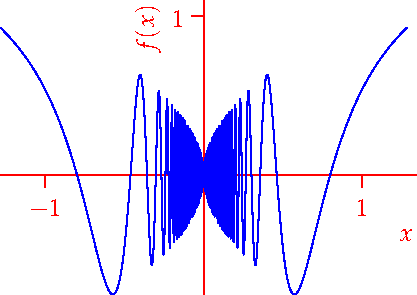
\includegraphics{cont-weird}
%   \end{minipage}
% 	\[0<\nm{x}<\delta\implies\nm{\sqrt{\nm x}\cos(1/x)-0}\le\sqrt{\nm x}<\sqrt\delta=\epsilon\]

		\item Let $f:\R\to\R$ be the \emph{indicator function} for the rational numbers:
		\[
			f(x)=
			\begin{cases}
				1&x\in\Q\\
				0&x\notin\Q
			\end{cases}
		\]
		Suppose $f$ is continuous at $a$ and let $\epsilon=1$. Then $\exists\delta$ such that 
		\[
			\nm{x-a}<\delta\implies \nm{f(x)-f(a)}<1 \tag{$\ast$}
		\]
		There are two cases; these rely on the fact that any interval contains both rational and irrational numbers (Corollary \ref{cor:qdense}, etc.).
		\begin{enumerate}
			\item If $a\in\Q$, then $f(a)=1$. There exists an irrational number $x\in(a-\delta,a+\delta)$, whence $\nm{f(x)-f(a)}=\nm{0-1}=1\not <1$.
			\item If $a\notin\Q$, then $f(a)=0$. There exists a rational number $x\in(a-\delta,a+\delta)$, whence $\nm{f(x)-f(a)}=\nm{1-0}=1\not <1$.
		\end{enumerate}
		Either way, we have contradicted ($\ast$). We conclude that $f$ is \emph{nowhere continuous.} 
	
		\item\label{ex:contonepoint} Let $g:\R\to\R$ be defined by
		\[
			g:\R\to\R:x\mapsto
			\begin{cases}
				x&x\in\Q\\
				0&x\notin\Q
			\end{cases}
		\]
		Since $0\le \nm{g(x)}\le \nm{x}$, the squeeze theorem tells us that $g$ is continuous at $x=0$.\smallbreak
		Now suppose $g$ is continuous at $a\neq 0$ and let $\epsilon=\nm a$. Then $\exists\delta$ such that
		\[
			\nm{x-a}<\delta\implies \nm{f(x)-f(a)}<\nm a
		\]
		The same two cases as in the previous example provide contradictions. We conclude that $g$ \emph{is continuous at precisely one point!}

\end{enumerate}

\end{examples}


\goodbreak

% \begin{description}
% 	\item[Definition + Limit Laws] Let $x_n\to a$, then
% 	\[\lim f(x)=\lim(3x_n^2-2)=3(\lim x_n)^3-2=3a^3-2=f(a)\]
% 	\item[Definition + Squeeze Theorem] Let $x_n\to a$. Then $\exists N$ such that $n>N\implies \nm{x_n-a}<1$. Now, for $n>N$,
% 	\begin{align*}
% 	\nm{f(x_n)-f(a)}&=\nm{3x_n^3-2-3a^3+2}=3\nm{x_n^3-a^3}=3\nm{x_n^2+ax_n+a^2}\nm{x_n-a}\\
% 	&<3\nm{(\nm a+1)^2+\nm a(\nm a+1)+a^2}\nm{x_n-a}=3(3a^2+3\nm a+1)\nm{x_n-a}
% \end{align*}
% 	Let $n\to\infty$ to see that $f(x_n)\to f(a)$.
% 	\item[Theorem \ref{thm:cont}] Let $\epsilon>0$ be given. Then let $\delta=\min\{\frac{\epsilon}{3(3a^2+3\nm a+1)},1\}$. By the above calculation,
% 	\[\nm{x-a}<\delta\implies \nm{f(x)-f(a)}\le 3(3a^2+3\nm a+1)\nm{x-a}< 3(3a^2+3\nm a+1)\delta\le\epsilon\]
% \end{description}



% \paragraph{Example}
% 
% Here is an example where we demonstrate discontinuity explicitly.\\[5pt]
% Show that $f(x)=\begin{cases}
% 	1&x\le 0\\
% 	3&x>0
% 	\end{cases}$\quad is discontinuous at $x=0$.
% 	\begin{description}
% 		\item[By the Definition] The sequence $x_n=\frac 1n$ has limit zero, however $f(x_n)=3\to 3\neq f(0)$.
% 		\item[By the Theorem (contradiction)] Suppose $f$ is continuous at $x=0$ and let $\epsilon=1$.	Then $\exists\delta$ such that\
% 		\[\nm{x-0}<\delta\implies \nm{f(x)-f(0)}=\nm{f(x)-1}<1\]
% 		But $f(\frac\delta 2)=3$ contradicts this.
% 		\item[By the Theorem (direct)]
% 		Let $\epsilon=1$, let $\delta>0$ be given and let $x=\frac\delta 2$. Then
% 		\[\nm{x-0}=\frac\delta 2<\delta\text{ and }\nm{f(x)-f(0)}=\nm{3-1}=2\ge \epsilon\]
% 	\end{description}


% 
% \begin{aside}
% 
% {\bf Aside: Continuity of Common Transcendental Functions}\\
% 
% A complete proof of Theorem \ref{thm:conttrig} is very difficult at this stage. It is much more efficient to wait until a good theory of power series and calculus has been developed. We can then define familiar functions as power series: e.g.,
% \[e^x=\sum_{n=0}^\infty\frac{x^n}{n!}\qquad \sin x=\sum_{n=0}^\infty\frac{(-1)^n}{(2n+1)!}x^{2n+1}\qquad \cos x=\sum_{n=0}^\infty\frac{(-1)^n}{(2n)!}x^{2n}\]
% Using the ratio test, it is easy to check that these series converge for \emph{any} real number $x$. General results then show that power series are continuous (and indeed differentiable term-by-term). It requires, of course, a little work to show that these definitions are equivalent to more familiar formulations.\\
% 
% There is, however, nothing stopping us from trying to establish the  continuity of these functions directly from the most basic definitions. For example, here is a sketch whereby the continuity of the sine function is established.
% \begin{enumerate}
%   \begin{minipage}[t]{0.55\linewidth}\vspace{0pt}
%   	\item If $x\in[0,\frac\pi 2)$, the definition of $\sin x$ and $\cos x$ comes from the picture. Since we are working in radians, the arc of the circle subtending  the angle $x$ is also $x$. The domains of sine and cosine may be continued to $\R$ in the usual periodic fashion.
% 	\item Prove the multiple-angle formula:
% 	\[\sin(a+b)=\sin a\cos b+\cos a\sin b\]
%   \end{minipage}\begin{minipage}[t]{0.45\linewidth}\vspace{0pt}
%   \flushright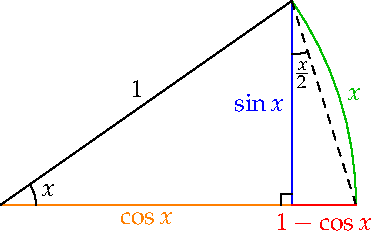
\includegraphics{trig-diff}
%   \end{minipage}\\[5pt]
% 	This has several elementary proofs: look one up!
% 	If $a$ is constant, and $b=x_n\to 0$, we see that to show continuity at $x=a$, it is enough for $\sin x_n\to 0$ and $\cos x_n\to 1$.
% 	\item From the picture we see that if $0\le x_n\le \frac\pi 2$, we have
% 	\[0\le\textcolor{blue}{\sin x_n}\le \textcolor{Green}{x_n}\quad\text{and}\quad 0\le\frac{\textcolor{red}{1-\cos x_n}}{\textcolor{Green}{x_n}}\le \sin\frac{x_n}2 \implies 1-x_n\sin\frac{x_n}2\le\cos x_n\le 1\]
% 	Two applications of the squeeze theorem complete the proof.\footnote{To be completely thorough, one needs also to consider sequences $x_n<0$ which converge to zero, then any sequence converging to zero will be bounded between a positive and negative convergent sequence. This is extremely tedious!} Since every trigonometric function can be defined in terms of sine (e.g. $\cos x=\sin(x+\frac\pi 2)$, $\tan x=\frac{\sin x}{\cos x}$, etc.), we see that all trigonometric function are continuous.
% 	\end{enumerate}
% 	
% It is somewhat trickier to prove the continuity of the exponential function directly from the only definition we've seen:
% \[\exp(x):=\lim_{n\to\infty}\left(1+\frac xn\right)^n\]
% Until integeration and power series are developed in a later course, we will simply assume that this function is continuous without proof.
% 	\begin{enumerate}
% 	  \item The only definition we have available pre-calculus is $\operatorname{Exp}(x):=\lim\left(1+\frac xn\right)^n$. This can be shown to converge for all $x\in\R$ similarly to how we defined $e=\lim\left(1+\frac 1n\right)^n$.
% 	  \item We now have to carefully show that $\operatorname{Exp}(x)=e^x$ really is an exponential function, so that $e^{x+y}=e^xe^y$, etc., that it is \emph{injective} and so has an inverse function $\ln x$.
% 	  \item As with sine, one can show continuity of $e^x$ if one can prove it at $x=0$. This is now easy using logarithms: given $\epsilon>0$, let $\delta=\ln(1+\epsilon)$. Then
% 	  \[\nm{x}<\delta\implies e^x\in(e^{-\delta},e^\delta)\implies \nm{e^x-1}<e^\delta-1=\epsilon\]
% 	\end{enumerate}\vspace{-25pt}
% \end{aside}

\goodbreak


\begin{exercisessec}{}{}
	\exstart Consider the function with $f(x)=\frac 1{\sqrt{x^2+2x-3}}$.\vspace{-2pt}
	\begin{enumerate}\setcounter{enumi}{1}
	  \item[]\begin{enumerate}
	    \item The implied domain of $f$ has the form $\dom f=(-\infty,a)\cup (b,\infty)$. Find $a$ and $b$.
	    \item What is the range of $f$?
	    \item Show that $f:(b,\infty)\to\operatorname{range}f$ is \emph{bijective} and compute its inverse function.
	    \item Find the inverse function when we instead restrict the domain to $(-\infty,a)$.
	    \item Briefly explain why $f$ is continuous on its domain.
	  \end{enumerate}
	  
  \item %[8.]sort of
  \label{exs:maxcont}
  Let $f$ and $g$ be continuous functions at $a$.
  \begin{enumerate}
    \item Show that $\max(f,g)=\frac 12(f+g)+\frac 12\nm{f-g}$ and deduce that $\max(f,g)$ is continuous at $a$. 
  	\item How might you show continuity of $\min(f,g)$?
  	%=-\max(-f,-g)$.
  \end{enumerate}
  

  
%   \item[2.] Let $f(x)=\begin{cases}
%   4&x\ge 0\\
%   0&x<0
%   \end{cases}$ and $g(x)=x^2$ for all $x$. Thus $\dom(f)=\dom(g)=\R$.
%   \begin{enumerate}
%   \item Determine the following functions: $f+g$, $fg$, $f\circ g$, $g\circ f$. Be sure to specify their domains.
%   \item Which of the functions $f$, $g$, $f+g$, $fg$, $f\circ g$, $g\circ f$ are continuous?
%   \end{enumerate}

  
  \item Use $\epsilon$--$\delta$ arguments to prove the following.
  \begin{enumerate}
  	\item $f(x)=x^2-3x$ is continuous at $x=1$
  	\item $g(x)=x^3$ is continuous at $x=a$.
  	\item $h:[0,\infty)\to\R:x\mapsto\sqrt x$ is continuous.
  	\item $j(x)=3x^{-1}$ is continuous on $\R\setminus\{0\}$.
  \end{enumerate}
  
 

	\item Prove that $x=0$ is a discontinuity of each function: use \emph{both} definitions of continuity.
	\begin{enumerate}
  	\item $f(x)=1$ for $x<0$ and $f(x)=0$ for $x\ge 0$.
  	\item $g(x)=\sin(1/x)$ for $x\neq 0$ and $g(0)=0$.
	\end{enumerate}


	\item Suppose $f$ and $g$ are continuous at $a$. Prove the following using $\epsilon$--$\delta$ arguments.
	\begin{enumerate}
  	\item $f-g$ is continuous at $a$.
  	\item If $h$ is continuous at $f(a)$, then $h\circ f$ is continuous at $a$.
	\end{enumerate}
	
  
%   \item Give examples to show that $g\circ f$ being continuous at $a$ can happen with:
%  	\begin{enumerate}
%     \item $g$ discontinuous at $a$ and $f$ continuous at $g(a)$.
%     \item $g$ continuous at $a$ and $f$ discontinuous at $g(a)$.
%     \item $g$ discontinuous at $a$ and $f$ discontinuous at $g(a)$.
%   \end{enumerate}
%   You may use pictures, but make sure they clearly describe the functions $f,g$.

	
  
  \item Suppose $f:U\to V\subseteq\R$ is a function whose domain $U$ contains an \emph{isolated point} $a$: i.e.\ $\exists r>0$ such that $(a-r,a+r)\cap U=\{a\}$. Prove that $f$ is continuous at $a$.
  

	\item In Example \ref*{ex:contesoteric}.\ref{ex:contonepoint}, provide the details of the required contradiction.
% 		\begin{enumerate}
% 		  \item Suppose $a$ is rational. Then $\exists x$ irrational for which $\nm{x-a}<\delta$, whence $\nm{f(x)-f(a)}=\nm{0-a}<\nm a$: contradiction.
% 		  \item Suppose $a$ is irrational. Then $\exists x$ rational for which $\nm{x-a}<\delta$ and $\nm a<\nm x<\nm a+\delta$. But then $\nm{f(x)-f(a)}=\nm{x-0}<\nm a$ is a contradiction.
%   	\end{enumerate}

	\item%[12]
	\begin{enumerate}
	  \item Suppose $f:\R\to\R$ is a continuous function for which $f(x)=0$ whenever $x\in\Q$. Prove that $f(x)=0$ for all $x\in\R$.
	  \item Suppose $f,g:\R\to\R$ are continuous functions such that $f(x)=g(x)$ for all rational $x$. Prove that $f=g$.  
	\end{enumerate}

	
	\item (Hard)\lstsp	Consider $f:\R\to\R$ where
	\[f(x)=\begin{cases}
	\frac 1q&\text{whenever }x=\frac pq\in\Q\text{ with }q>0\text{ and }\gcd(p,q)=1\\
	0&\text{ if }x\not\in\Q
	\end{cases}\]
  For example, $f(1)=f(2)=f(-7)=1$, and $f(\tfrac 12)=f(-\tfrac 12)=f(\tfrac 32)=\cdots=\frac 12$, etc. Prove that $f$ is continuous at each irrational number, and discontinuous at each rational number.	
  	
  	
\end{enumerate}
\end{exercisessec}

\clearpage



\section{Properties of Continuous Functions}

\def\range{\operatorname{range}}

In this section consider how continuous functions transform \emph{intervals.}

\begin{example}[lower separated=false, sidebyside, sidebyside align=top seam, sidebyside gap=0pt, righthand width=0.3\linewidth]{}{propcont1}
	$f(x)=x^2$ maps $\textcolor{Green}{[-3,2]}$ onto $\textcolor{magenta}{[0,9]}$. In particular:
	\begin{itemize}\itemsep0pt
	  \item $f$ transforms one \textcolor{Green}{interval} into \textcolor{magenta}{another}.
	  \item $f$ transforms one \textcolor{Green}{closed bounded set} into \textcolor{magenta}{another}.
	\end{itemize}
	The purpose of this section is to see that these are general properties exhibited by \emph{any} continuous function. 
	\tcblower
	\flushright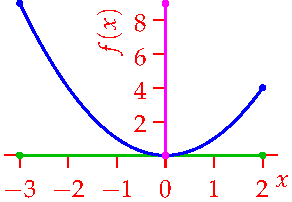
\includegraphics[scale=0.9]{properties-ex1}
\end{example}


	Before stating our first result, recall a couple of definitions.

\begin{defn}{}{}
Let $U,V\subseteq\R$ and $f:U\to V$.
	\begin{enumerate}
	  \item\begin{enumerate}
	    \item $U$ is \emph{bounded} if $\exists M$ such that $\forall x\in U, \nm{x}\le M$.
	    \item $f$ is \emph{bounded} if its range is a bounded set: $\exists M\text{ such that }\forall x\in U,\ \nm{f(x)}\le M$.
	  \end{enumerate}
	  \item (Definition \ref{defn:closed}) $U$ is \emph{closed} if every convergent sequence in $U$ has its limit in $U$:
		\[\forall (x_n)\subseteq U,\ \lim x_n=s\ (\in\R)\implies s\in U\]
	\end{enumerate}
\end{defn}

\begin{thm}{Extreme Value Theorem}{extremevalue}
	Suppose $f:U\to V$ is continuous where $U$ is closed and bounded. Then $f$ is bounded and attains its bounds: %($\range f$ is closed and bounded):
	\[
		\exists s,i\in U\quad \text{such that}\quad f(s)=\sup\bigl(f(U)\bigr)\quad\text{and}\quad	f(i)=\inf\bigl(f(U)\bigr)
	\]
	In fact $f(U)$ is also closed and bounded.
\end{thm}

In Example \ref{ex:propcont1}, if $U=[-3,2]$, then $s=-3$ and $i=0$.

\begin{examples}{}{}
	Before seeing the proof, here are three examples where we weaken one of the hypotheses and see that the result fails.
	\begin{center}
	\begin{tabular}{c@{\qquad}c@{\qquad}c}
		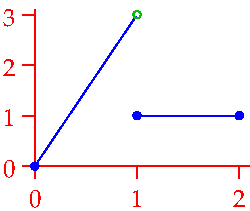
\includegraphics[scale=0.95]{extreme2}
		&
		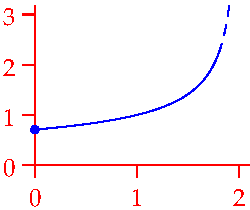
\includegraphics[scale=0.95]{extreme3}
		&
		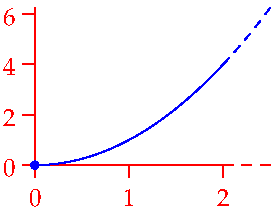
\includegraphics[scale=0.95]{extreme4}
		\\
		1. \ $f$ discontinuous
		&
		2. \ $U$ not closed
		&
		3. \ $U$ not bounded	
	\end{tabular}
	\end{center}
	\smallskip
	
	\begin{enumerate}
	  \item $\sup(\range f)=3$ is not attained by $f(x) =\smash{\begin{cases}
	  3x&\text{if }0\le x<1\\
	  1&\text{if }1\le x\le 2
	  \end{cases}}$\smallskip
	  \item If $f(x)=\frac 1{\sqrt{2-x}}$ and $U=[0,2)$, then $\range f=[\frac 1{\sqrt 2},\infty)$ is unbounded.
	  \item If $f(x)=x^2$ and $U=[0,\infty)$, then $\range f=[0,\infty)$ is unbounded.
	\end{enumerate}
\end{examples}

\goodbreak

The goal of the proof is to show that every limit point of $f(U)=\range f$ lies in $f(U)$. The proof is broken into simple steps: observe where each hypothesis is used.

\begin{proof}
\begin{enumerate}\itemsep2pt
  \item Suppose $M$ is a limit point of $f(U)$: that is, $M=\lim\bigl(f(x_n)\bigr)$ for some sequence $(x_n)\subseteq U$.	\emph{A priori} $M$ need not be finite, but it is possible\footnotemark{} that $M=\sup\bigl(f(U)\bigr)$ or $\inf\bigl(f(U)\bigr)$.
	\item Since $(x_n)\subseteq U$ is \emph{bounded,} Bolzano--Weierstraß (Theorem \ref{thm:bolzano}) says it has a convergent subsequence, $\lim\limits_{k\to\infty}x_{n_k}=x$.
	\item	Since $U$ is \emph{closed,} we have $x\in U$. This means $f(x)$ makes sense (it is a \emph{real number}!).
	\item	Since $f$ is \emph{continuous,} we have $\lim f(x_{n_k})=f(x)$.
	\item	Finally, $M=f(x)$ since all subsequences of a convergent (or divergent to $\pm\infty$) sequence tend to the same limit (Lemma \ref{lemm:subseqconv}). It follows that all limit points $M$ are \emph{finite} and lie in $f(U)$: otherwise said, $f(U)$ is closed and bounded.
\end{enumerate}
\medskip
In particular, choosing $M=\sup\bigl(f(U)\bigr)$ yields $x=s\in U$ as in the Theorem.
\end{proof}


% \begin{proof}
% 	Let $M=\sup\bigl(\range f\bigr)$: \emph{a priori} this could be infinite! We break the proof into several steps; note where we use each of the hypotheses regarding $f$.
% 	\begin{enumerate}
% 	  \item There exists\footnotemark{} a sequence $(x_n)\subseteq U$ such that $\lim f(x_n)=M$.
% 	  \item	Since $(x_n)\subseteq U$ is \emph{bounded,} Bolzano--Weierstraß (Theorem \ref{thm:bolzano}) says it has a convergent subsequence, $\lim\limits_{k\to\infty}x_{n_k}=s$.
% 	  \item	Since $U$ is \emph{closed,} we have $s\in U$.
% 	  \item	Since $f$ is \emph{continuous,} we have $\lim f(x_{n_k})=f(s)$.
% 	  \item	Finally, $M=f(s)$ since all subsequences of a convergent sequence converge to the same limit (Lemma \ref{lemm:subseqconv}). In particular, $M$ must now be \emph{finite}, and so $\range f$ is bounded above.
% 	\end{enumerate}
% 	The discussion for the infimum is similar.
% \end{proof}

\footnotetext{If $M=\sup\bigl(f(U)\bigr)$, then a suitable $(x_n)$ might be constructed as follows:
	\begin{itemize}
    \item If $M\in\R$, then for each $n\in\N,\exists x_n\in U$ such that $M-\frac 1n<f(x_n)\le M$ (Lemma \ref{lemm:contrasup}).
		\item If $M=\infty$, then for each $n\in\N,\exists x_n\in U$ such that $f(x_n)\ge n$.
  \end{itemize}}

\begin{example}{}{oddpolyroot}
	It is worth thinking about why we needed to use a \emph{subsequence} in the proof. The reason is that it is possible for the bounds of $f$ to be attained multiple times. For example, consider
	\[
		f:[0,4\pi]\to\R:x\mapsto \sin x
	\]
	This satisfies the hypotheses of the extreme value theorem: $[0,4\pi]$ is closed and bounded and $f$ is continuous. Indeed $\max(\range f)=1$ is attained at \emph{both} $x=\frac\pi 2$ and $\frac{5\pi}2$. The sequence defined by
	\[
		x_n=
		\begin{cases}
			\frac\pi 2+\frac 1n&\text{if $n$ odd}\\
			\frac{5\pi}2+\frac 1n&\text{if $n$ even}
		\end{cases}\quad\text{has}\quad f(x_n)=\sin\left(\frac\pi 2+\frac 1n\right)\xrightarrow[n\to\infty]{} 1 =\sup(\range f)
	\]
	and therefore satisfies step 1 of the proof. However, $(x_n)$ itself is \emph{divergent by oscillation.} Bolzano--Weierstraß is used to force the existence of a convergent subsequence; in this case the subsequence of odd terms $(x_{n_k})=(x_{2k-1})$ satisfies the remaining steps of the proof.
	\begin{center}
		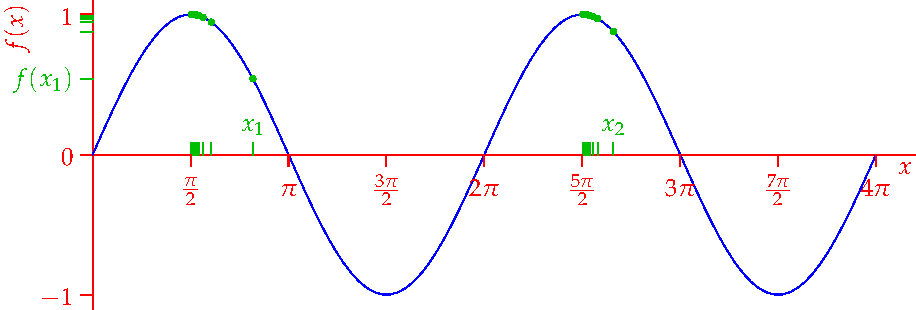
\includegraphics[scale=0.95]{extval}
	\end{center}
\end{example}

\goodbreak


\boldsubsubsection{The Intermediate Value Theorem and its Consequences}

This result should be familiar from elementary calculus, even if its proof is not! It is also intuitive: if you climb a hill, then at some point you must be half-way up the hill\ldots


\begin{thm}{Intermediate Value Theorem (IVT)}{}
	Let $f$ be continuous on the interval $[a,b]$ and let $y$ lie strictly between $f(a)$ and $f(b)$. Then $\exists\xi\in(a,b)$ such that $f(\xi)=y$.
\end{thm}



\begin{proof}
	WLOG assume $f(a)<y<f(b)$. Now let $S=\{x\in[a,b]:f(x)<y\}$ and \emph{define} $\textcolor{Green}{\xi:=\sup S}$.\par
	\begin{minipage}[t]{0.51\linewidth}\vspace{0pt}
		Since $S$ is non-empty ($a\in S$) and bounded above (by $b$), we see that $\xi$ exists and is finite. It remains to prove that $a<\xi<b$ and $f(\xi)=y$.\smallbreak
		First choose any $\textcolor{Brown}{(s_n)}\subseteq S$ such that\footnotemark{} $\lim\textcolor{Brown}{s_n}=\textcolor{Green}{\xi}$.
		Continuity forces $\lim f(\textcolor{Brown}{s_n})=f(\textcolor{Green}{\xi})$. Moreover
		\[
			f(\textcolor{Brown}{s_n})\le y\implies f(\textcolor{Green}{\xi})\le y
		\]
		This also shows that $\xi<b$.
	\end{minipage}
	\hfill
	\begin{minipage}[t]{0.48\linewidth}\vspace{0pt}
		\hfill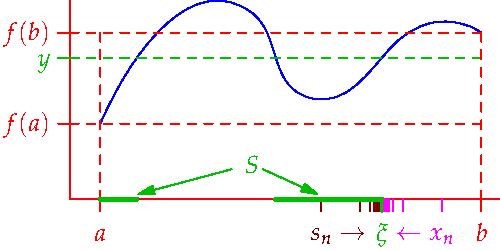
\includegraphics[scale=0.95]{intval}
	\end{minipage}
	\smallbreak
	We now play a similar game from the other side: define $\textcolor{Magenta}{x_n}:=\min(\xi+\frac 1n,b)$, then $\lim\textcolor{Magenta}{x_n}=\textcolor{Green}{\xi}$ and $\textcolor{Magenta}{x_n}>\textcolor{Green}{\xi}=\sup S\implies \textcolor{Magenta}{x_n}\not\in S$, whence
  \[
  	f(\textcolor{Magenta}{x_n})\ge y\implies f(\textcolor{Green}{\xi})=\lim f(\textcolor{Magenta}{x_n})\ge y
  \]
  This also shows that $\xi>a$. Putting it all together, we conclude that $f(\xi)=y$ and $\xi\in(a,b)$.
\end{proof}

\footnotetext{Similarly to step 1 of the proof of the Extreme Value Theorem.}

Note how the value of $\xi$ in the proof is always the \emph{largest} of potentially several choices.\smallbreak



\begin{examples}{}{}
	The intermediate value theorem was typically used in elementary calculus to show the existence of solutions to equations. Here are a couple of examples of this process.
	\begin{enumerate}
	  \item We show that the equation $x^7+3x=1+4\cos(\pi x)$ has a solution.\smallbreak
		The trick is to express the equation in the form $f(x)=y$ where $f$ is continuous, then choose suitable $a,b$ to fit the theorem. In this case,
		\[f(x)=x^7+3x-4\cos(\pi x)\quad\text{and}\quad y=1\]
		are suitable choices. Now observe that
		\[f(0)=-4<y\quad\text{and}\quad f(1)=1+3+4=8>y \tag{i.e., $a=0$ and $b=1$}\]
		whence $\exists\xi\in(0,1)$ such that $f(\xi)=01$. Otherwise said, $\xi$ is a solution to the original equation.\smallbreak
		The function $f$ is in fact continuous on $\R$, a much larger interval that $[a,b]$, but no matter!
		
		\goodbreak
		
		
	\begin{minipage}[t]{0.7\linewidth}\vspace{0pt}
		\item\label{ex:oddpolyroot2} The existence of a root $\xi$ of the (continuous) polynomial
		\[
			f(x)=x^5-5x^4+150
		\]
		follows from the intermediate value theorem by observing that
		\[
			f(0)=150>0\quad\text{and}\quad f(4)=-256+150=-106<0
		\]
		We conclude that such a root exists and that $\xi\in(0,4)$.\par
		As the graph suggests, there are other roots ($\textcolor{Magenta}{\eta,\zeta}$), the existence of which may be shown by also evaluating, say,
		\[
			f(-3)=-798<0\quad\text{and}\quad f(5)=150>0
		\]
		%For greater accuracy of estimation, we need only evaluate $f$ at more places and apply the theorem again.
	\end{minipage}\begin{minipage}[t]{0.3\linewidth}\vspace{0pt}
		\flushright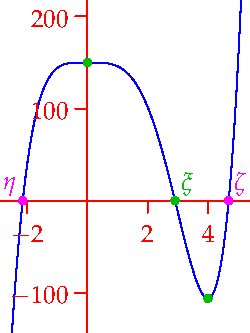
\includegraphics[scale=0.9]{intval2}
	\end{minipage}
	\smallbreak

		With an eye on generalizing, consider a slightly different approach. Define two sequences $(s_n)$ and $(t_n)$ via
		\[
			s_n:=\frac{f(-n)}{n^5} =-1-\frac{5}n+\frac{150}{n^5}
			\qquad
			t_n:=\frac{f(n)}{n^5}= 1-\frac{5}n+\frac{150}{n^5}
		\]
		Since $\lim s_n=-1$ and $\lim t_n=1$,  we see that
		\begin{gather*}
			\exists a\text{ such that }s_a<-\frac 12\implies f(-a)=a^5s_a<-\frac 12a^5<0\\
			\exists b\text{ such that }t_b>\frac 12\implies f(b)=b^5t_b>\frac 12b^5>0
		\end{gather*}
		Applying the intermediate value theorem on $[-a,b]$ shows the existence of a root.
	\end{enumerate}
\end{examples}

The second approach in Example \ref*{ex:oddpolyroot}.\ref{ex:oddpolyroot2} may be applied to prove the general result.

\begin{cor}{}{odddegreepolyroot}
	A polynomial function of odd degree has at least one real root.
\end{cor}


The proof is an exercise. An even simpler exercise shows the existence of a \emph{fixed point} for a particular type of continuous function. 


\begin{cor}{Fixed Point Theorem}{fixedpoint}
	Suppose $a$ and $b$ are finite and that $f:[a,b]\to [a,b]$ is continuous. Then $f$ has a fixed point:
	\[\exists\xi\in[a,b]\text{ such that }f(\xi)=\xi\]
\end{cor}

\begin{minipage}[t]{0.7\linewidth}\vspace{0pt}
	As the picture shows, a function could have several fixed points.\smallbreak
	This is the first of several fixed-point theorems you'll meet if your studies of analysis continue. Many important consequences flow from these, including a common fractal construction and the standard existence/uniqueness result for differential equations. 
\end{minipage}
\hfill
\begin{minipage}[t]{0.29\linewidth}\vspace{0pt}
	\flushright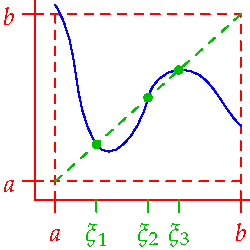
\includegraphics[scale=0.95]{intval3}
\end{minipage}


\goodbreak

For our final corollary, we first note a straightforward characterization% which helps us deal with all intervals simultaneously
: a set $I\subseteq\R$ is an interval if
\[a,b\in I \text{ and }\ a<y<b\implies y\in I\tag{$\ast$}\]

\begin{cor}{Preservation of Intervals}{}
	Suppose $f:U\to V$ is continuous where $U=\dom f$ is an interval (of positive length) and $V=\range f$.\vspace{-1pt}
	\begin{enumerate}\itemsep0pt
	  \item $V$ is an interval or a point.
	  \item If $f$ is strictly increasing (decreasing), then:\vspace{-3pt}
		\begin{enumerate}
		  \item $V$ is an interval (it has positive length).
		  \item $f$ is \emph{injective} (and thus bijective).
		  \item The inverse function $f^{-1}:V\to U$ is also continuous and strictly increasing (decreasing).
		\end{enumerate}
	\end{enumerate}
\end{cor}

\begin{example}[lower separated=false, sidebyside, sidebyside align=top seam, sidebyside gap=0pt, righthand width=0.3\linewidth]{}{}
	In part 1, note that the interval $V$ \emph{need not be of the same type} as $U$. For instance, if $f(x)=10x-x^2$, then $f$ maps the \emph{open} interval $U=(2,9)$ to the \emph{half-open} interval $V=(9,25]$.\smallbreak
	The extreme value theorem, however, guarantees that if $U$ is a closed bounded interval, then $V$ is also, for instance,
	\[
		f\bigl([2,9]\bigr)=[9,25]
	\]
	\tcblower
	\flushright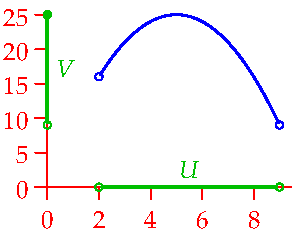
\includegraphics[scale=0.95]{intval4}
\end{example}


\begin{proof}
\begin{enumerate}
  \item If $V$ is not a point, then $\exists a,b\in U$ such that $f(a)<f(b)$. Let $y\in\bigl(f(a),f(b)\bigr)$; IVT says $\exists\xi$ between $a$ and $b$ such that $y=f(\xi)$. That is, $y\in \range f$. By ($\ast$), $V=\range f$ is an interval.
  \item\begin{enumerate}
    \item[(a,b)] If $f$ is strictly increasing, then $\forall a,b\in U,\ a<b\implies f(a)<f(b)$. It follows that $f$ is injective and that $V$ contains at least 2 points; by part 1 it has positive length.
    \item[(c)] Let $y_1<y_2$ where both lie in $V$, and define $x_i=f^{-1}(y_i)$ for $i=1,2$. Since $f$ is increasing,
		\[
			x_2\le x_1\implies y_2=f(x_2)\le f(x_1)=y_1
		\]
		is a contradiction. Thus $x_1<x_2$ and $f^{-1}$ is also strictly increasing.\par
		It remains to show that $f^{-1}$ is continuous at $b=f^{-1}(a)$. Assume first that $a$ is not an endpoint of $U$. Given $\epsilon>0$ for which $[\textcolor{Brown}{a-\epsilon},\textcolor{Magenta}{a+\epsilon}]\subseteq U$, let
		\[\delta:=\min\bigl(\textcolor{Brown}{b-f(a-\epsilon)},\textcolor{Magenta}{f(a+\epsilon)-b}\bigr)\]
		and observe that
		\begin{align*}
			\nm{y-b}<\delta&\implies \textcolor{Brown}{f(a-\epsilon)-b}<y-b<\textcolor{Magenta}{f(a+\epsilon)-b}%\\
			%&
			\implies f(a-\epsilon)<y<f(a+\epsilon)\\
			&\implies a-\epsilon<y<a+\epsilon \tag{$f$ strictly increasing}\\
			&\implies \nm{f^{-1}(y)-a}<\epsilon
		\end{align*}
		If $a$ is an endpoint of $U$, instead use $\textcolor{Brown}{[a-\epsilon,a]\subseteq U}$ or $\textcolor{Magenta}{[a,a+\epsilon]\subseteq U}$ and only the corresponding half of the expression $\delta$.\qedhere
  \end{enumerate}
\end{enumerate}
\end{proof}


\goodbreak

\begin{example}[lower separated=false, sidebyside, sidebyside align=top seam, sidebyside gap=0pt, righthand width=0.3\linewidth]{}{nondiffinverse}
	The function $f:[0,2]\to[0,4]$ defined by
	\[
		f(x)=
		\begin{cases}
			\sqrt[3]{x}&\text{if }0\le x\le 1\\
			x^2&\text{if }1<x\le 2
		\end{cases}
	\]
	is continuous and strictly increasing. It therefore has a continuous inverse function $f^{-1}:[0,4]\to[0,2]$.\smallbreak
	Compare this with the result from elementary calculus: $f'>0\implies f$ injective. We cannot apply this here since $f$ is not differentiable!
	\tcblower
	\flushright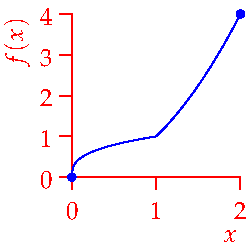
\includegraphics{inversecont}
\end{example}


\begin{exercisessec}{}{}
\exstart Give an example of a \emph{discontinuous} function $f:[0,1]\to\R$ which is \emph{not bounded.}
\begin{enumerate}\setcounter{enumi}{1}
  \item Let $a<b$ be given. Give examples of \emph{continuous} functions $g,h:(a,b)\to\R$ such that:
	\begin{enumerate}
		 \item $g$ is \emph{not bounded.}
		 \item $h$ is bounded but \emph{does not attain its bounds.}
	\end{enumerate}
	
%   \item Recalling elementary calculus (derivative tests), the function $f:[-\sqrt 3,\sqrt 3]\mapsto \R:x\mapsto x^3-3x$ has
%   \[\max f=2=f(-1),\qquad\min f=-2=f(1)\]
  
  \item Compute the inverse of the function $f$ in Example \ref{ex:nondiffinverse}.
  
  \item%[4.]* 
  Let $S\subseteq\R$ and suppose there exists a sequence $(x_n)$ in $S$ that converges to a number $x_0\not\in S$. Show that there exists an unbounded continuous function on $S$.
  
  \item%[6.]
  Prove that $x=\cos x$ for some $x$ in $(0,\tfrac\pi 2)$.
  
  \item%[8.]
  Suppose that $f$ is a real-valued continuous function on $\R$ and that $f(a)f(b)<0$ for some $a,b\in\R$. Prove that there exists $x$ between $a,b$ such that $f(x)=0$.
  
  \item%[10.]*
  Suppose that $f$ is continuous on $[0,2]$ and that $f(0)=f(2)$. Prove that there exist $x,y\in[0,2]$ such that $\nm{y-x}=1$ and $f(x)=f(y)$.\par
  (\emph{Hint: consider $g(x)=f(x+1)-f(x)$ on $[0,1]$})
  
  
  
 	\item\begin{enumerate}
 	  \item Prove the fixed point theorem (Corollary \ref{cor:fixedpoint}).\par
 	  (\emph{Hint: If neither $a$ nor $b$ are fixed points, consider $g(x)=f(x)-x$}) 
 	  
 	  \item Prove Corollary \ref{cor:odddegreepolyroot} for a general odd-degree monic polynomial $f(x)=x^{2m+1}+\sum\limits_{k=0}^{2m}\alpha_kx^k$. 
 	\end{enumerate}
 	

	
	\item Consider $f:\R\to\R$ where $f(x)=x\sin\frac 1x$ if $x\neq 0$ and $f(0)=0$.
	\begin{enumerate}
	  \item Explain why $f$ is continuous on any interval $U$.
	  \item Suppose $a<0<b$ and that $f(a),f(b)$ have opposite signs. If $y=0$, show that the intermediate value theorem is satisfied by \emph{infinitely many} distinct values $\xi$.
	\end{enumerate}
	%there are infinitely many $f(\xi)=0$ for \emph{infinitely}whenever $x=0,\pm\frac 1{n\pi}$ for any $n\in\N$.
	
	
	\item\begin{enumerate}
	  \item Suppose $f:U\to\R$ is continuous and that $U=\bigcup\limits_{k=1}^nI_k$ is the union of a finite sequence $(I_k)$ of closed bounded intervals. Prove that $f$ is bounded and attains its bounds.
	  \item Let $U=\bigcup\limits_{n=1}^\infty I_n$, where $I_n=[\frac 1{2n},\frac 1{2n-1}]$ for each $n\in\N$. Give an example of a continuous function $f:U\to\R$ which is either unbounded or does not attain its bounds. Explain.
	\end{enumerate}
	(\emph{This is related to the idea that \underline{finite} unions of closed sets remain closed, but \underline{infinite} unions need not})
\end{enumerate}
\end{exercisessec}

\clearpage


\section{Uniform Continuity}\label{sec:uniformcont}

Suppose $f:U\to V$ is continuous. By the $\epsilon$-$\delta$ definition (\ref{defn:epcont}),
\[
	\textcolor{blue}{\forall a\in U},\ \forall \epsilon>0,\ \exists \delta(a,\epsilon)>0\text{ such that }(\textcolor{blue}{\forall x\in U})\ \nm{x-a}<\delta\implies\nm{f(x)-f(a)}<\epsilon\tag{$\ast$}
\]
We write $\delta(a,\epsilon)$ to stress the fact that $\delta$ can depend both on the \emph{location} $a$ and the \emph{distance} $\epsilon$. The goal of this section is to understand if/when it is possible to choose $\delta$ \emph{independently of the location $a$.}

\begin{example}{}{unif01}
	We start by considering how this desire might be impossible to satisfy.\par
	\begin{minipage}[t]{0.6\linewidth}\vspace{-3pt}
		Consider $f(x)=x^2$ with domain $U=[0,\infty)$. Given $\epsilon>0$ and $a_1\in U$, we can certainly find some\footnotemark{} $\delta$ such that
		\[
			\textcolor{Green}{\nm{x-a_1}<\delta}\implies \textcolor{Magenta}{\nm{f(x)-f(a_1)}=\nm{x^2-a_1^2}<\epsilon}
		\]
		Visualize what happens if we try to use the \emph{same} $\delta$ for different $a_i$: imagine sliding the fixed-width \textcolor{Green}{$\delta$-interval} along the $x$-axis while simultaneously sliding the \textcolor{Magenta}{$\epsilon$-interval} vertically. As $a_i$ increases, the \textcolor{Green}{image} of the $\delta$-interval eventually becomes too large for the \textcolor{Magenta}{$\epsilon$-interval} to contain:
		\[
			\text{length}\bigl(f(a_i-\delta,a_i+\delta)\bigr) =(a_i+\delta)^2-(a_i-\delta)^2=4a_i\delta
		\]
		\emph{increases unboundedly} with $a_i$.
	\end{minipage}
	\hfill
	\begin{minipage}[t]{0.39\linewidth}\vspace{0pt}
		\flushright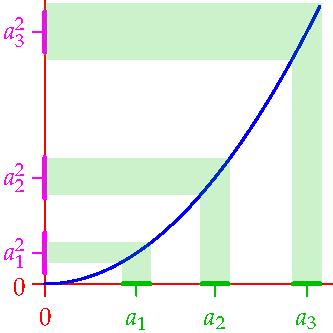
\includegraphics{unifcont}
	\end{minipage}\smallbreak
	
	For fixed $\epsilon$, as $a$ increases, the increasing \emph{gradient} of $f$ means that we need to choose a \emph{smaller} $\delta$.\medbreak
	
	By contrast, if we consider the same formula $f(x)=x^2$ but on a restricted \emph{finite} domain $[0,b]$, then any $\delta$ that suffices to demonstrate continuity at $x=b$ will also do so everywhere else on $[0,b]$. We'll check this explicitly in a moment.
\end{example}

\footnotetext{For instance $\delta =\min(1,\frac\epsilon{1+2a_1})$, as we saw on page \pageref{thm:cont}.}

To formalize things, consider rewriting ($\ast$), where we additionally assume that $\delta$ may be chosen independently of the location $a$; this amounts simply to moving the quantifier $\textcolor{blue}{\forall a\in U}$ after $\delta$.

\begin{defn}{}{}
	A function $f:U\to V\subseteq \R$ is \emph{uniformly continuous} if
	\[
		\forall\epsilon>0,\ \exists\delta>0\text{ such that }(\textcolor{blue}{\forall x,y\in U})\ \nm{x-y}<\delta\implies\nm{f(x)-f(y)}<\epsilon \tag{$\dag$}
	\]
\end{defn}

For reasons of symmetry we use $y$ instead of $a$. Note how $\delta$ now depends only on $\epsilon$ since it is quantified \emph{before} $x$ and $y$; as previously, the quantifiers for $x,y$ are usually hidden. Note also how uniform continuity is only relevant on the entire domain $U$; it makes no sense to speak of uniform continuity at a point $a$.
\smallbreak
For the sake of tidiness, we make one more observation before seeing some examples.

\begin{lemm}{}{}
	If $f$ is uniformly continuous on $U$, then it is continuous on $U$.
\end{lemm}

This should be trivial: $(\dag)$ is the $\epsilon$-$\delta$ continuity of $f$ at $y\in U$, \emph{for all $y$ simultaneously}! The special feature of the definition is that the same $\delta$ works for all $y$.

\goodbreak


\begin{examples}{}{unifeasy}
	\exstart We re-analyze $f(x)=x^2$ in view of the definition. Recall first that
	\[\nm{f(x)-f(y)}=\nm{x^2-y^2}=\nm{x-y}\nm{x+y}\]
	where $\nm{x-y}$ is easily controlled by $\delta$. We consider the behavior of $\nm{x+y}$ in two cases.
	\begin{enumerate}\setcounter{enumi}{1}
  \item[]\begin{description}
  	\item[Bounded domain] If $U=\dom f\subseteq [-T,T]$ for some $T>0$, we show that $f$ is uniformly continuous. This follows because $\nm{x+y}\le 2T$ is also easily controlled.\par
  	Let $\epsilon>0$ be given and define $\delta =\frac\epsilon{2T}$, then
		\[\nm{x-y}<\delta\implies \nm{f(x)-f(y)}<\delta\cdot 2T=\epsilon\]
		Compare with Example \ref{ex:unif01}. Our approach works for \emph{this} function because the gradient (and therefore potential discrepancy between $x^2-y^2$ and $x-y$) is greatest at the endpoints of the interval. The same approach may not work for other functions!

		\item[Unbounded domain] We show that $f$ is not uniformly continuous when $\dom f=[0,\infty)$.\par	
		For contradiction, assume $f$ is uniformly continuous: let $\epsilon=1$ and suppose $\delta>0$ satisfies the definition. Supposing $x-y=\frac\delta 2$, we see that
		\[\nm{x+y}=2y+\frac\delta 2 \implies	\nm{f(x)-f(y)}=\frac\delta 2\left(2y+\frac\delta 2\right) =\delta\left(y+\frac\delta 4\right)>\delta x\]
		Letting $y=\frac 1\delta$ \ ($x=\frac 1\delta+\frac\delta 2$) yields the contradiction $\nm{f(x)-f(y)}>1=\epsilon$.
	\end{description}
	
	\item Let $g(x)=\frac 1x$; we again consider two domains.\par
	\begin{minipage}[t]{0.65\linewidth}\vspace{-8pt}
	\begin{description}
		\item[Uniform continuity] on $[a,b)$ whenever $0<a<b\le \infty$.\par
		Let $\epsilon>0$ be given and let $\delta=a^2\epsilon$. Then,
		\begin{align*}
			\nm{x-y}<\delta \implies \nm{g(x)-g(y)}&=\nm{\frac{y-x}{xy}}\\
			&<\frac\delta{xy}\le\frac{\delta}{a^2}=\epsilon
		\end{align*}
		where the last inequality follows because $x,y\ge a$.
		\item[Non-uniform continuity] on $(0,b)$ whenever $0<b\le\infty$.\par
		As before, let $\epsilon=1$ and suppose $\delta>0$ is given. 
		Let
		\[x=\min\left(\delta,1,\frac b2\right) \quad\text{and}\quad y=\frac x2\]
		\makebox[0cm][l]{Certainly $x,y\in(0,b)$ and $\nm{x-y}=\frac x2\le\frac\delta 2<\delta$. However,}
		\[\nm{f(x)-f(y)}=\frac 1x\ge 1=\epsilon\]
	\end{description}
	\end{minipage}
	\hfill
	\begin{minipage}[t]{0.34\linewidth}\vspace{0pt}
		\flushright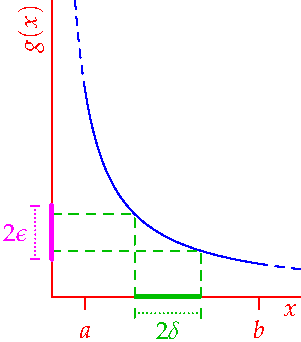
\includegraphics{unifcont2}
	\end{minipage}\bigbreak
Think about how $\epsilon$ and $\delta$ must relate as one slides the intervals in the picture up/down and left/right. In this case, large values of $x,y$ are not the problem, it's the vertical asymptote at zero that causes trouble. 
	
\end{enumerate}
\end{examples}


% 
% 	\begin{itemize}
% 	  \item Let $\epsilon>0$ be given; we'd like to find $\delta>0$ such that
% 		\[\nm{x-a}<\delta\implies\nm{x^2-a^2}<\epsilon\]
% 		Since\footnote{Recall that we're fixing the domain to be $[0,\infty)$ to keep calculations simpler. Without this restriction, the forthcoming function $M(a,\delta)$ is messier.} $\nm{x^2-a^2}=\nm{x-a}\nm{x+a}=\nm{x-a}(x+a)$, the challenge is to get a handle on the size of $x+a$. The best we can say is that
% \begin{align*}
% \nm{x-a}<\delta&\implies a-\delta<x<a+\delta\\
% &\implies 2a-\delta<x+a<2a+\delta\\
% &\implies \nm{x+a}<M(a,\delta):=2a+\delta\\
% &\implies\nm{x^2-a^2}=\nm{x-a}\nm{x+a}<\delta M
% \end{align*}
% It is enough to choose $\delta$ small enough so that $\delta M(a,\delta)\le\epsilon$.
% Any suitable choice of $\delta$ seems to depend on $a$, e.g.
% \[\delta=\min\left\{1,\frac{\epsilon}{M(a,1)}\right\}\quad\text{or}\quad \delta=\sqrt{a^2+\epsilon}-a\]
% 	\end{itemize}
 	
\boldsubsubsection{General Conditions for Uniform Continuity}

For the remainder of this section, we develop a few general ideas related to uniform continuity. The first is a little out of order since it depends on differentiation and the mean value theorem.

\begin{thm}{}{unifbddderiv}
	Suppose $f$ is continuous on an interval $U$ (finite or infinite) and differentiable except perhaps at its endpoints. If $f'$ is bounded, then $f$ is uniformly continuous on $U$.
\end{thm}

\begin{proof}
	Suppose $\nm{f'(x)}\le M$. Let $\epsilon>0$ and $\delta=\frac\epsilon M$. 
	% By the Mean Value Theorem, 
	Then
	\[\nm{x-y}<\delta\implies \nm{f(x)-f(y)}=\nm{f'(\xi)}\nm{x-y}<M\delta=\epsilon\]
	where the existence of $\xi$ between $x,y$ follows from the Mean Value Theorem.\footnotemark{}
\end{proof}

\footnotetext{If $x<y$ then $\exists \xi\in (x,y)$ such that $f'(\xi)=\dfrac{f(x)-f(y)}{x-y}$.}

\begin{examples}{}{}
	\exstart Compare the arguments in the previous exercise. For instance, if $\dom f\subseteq[-T,T]$,
	\[f(x)=x^2\implies f'(x)=2x\implies \nm{f'(x)}\le 2T\]
	The derivative is bounded, whence $f$ is uniformly continuous on $[-T,T]$.
	\begin{enumerate}\setcounter{enumi}{1}
	  \item Any polynomial is uniformly continuous on any bounded interval.
	  \item The function $f(x)=\sin x$ is uniformly continuous on $\R$ since $f'(x)=\cos x$ is bounded (by 1).
	  \item Consider $f(x)=\frac 1x-\frac 5{x^2}$ on $(1,\infty)$. We have
	  \[
	  	f'(x)=-\frac 1{x^2}+\frac{10}{x^3}\implies \nm{f'(x)}\le 11
	  \]
	  We conclude that $f$ is uniformly continuous on $(1,\infty)$.\smallbreak
	  The approach is often useful when you are asked to show \emph{using the definition} that a function is uniformly continuous; provided $f'$ is bounded by $M$, you may always choose $\delta=\frac\epsilon M$ to obtain an argument. For instance, with our function:\par
	  Given $\epsilon>0$, let $\delta=\frac\epsilon{11}$. If $x,y\in(1,\infty)$ and $\nm{x-y}<\delta$, then
	  \begin{align*}
	  	\nm{f(x)-f(y)} &=\nm{\frac 1x-\frac 1y+\frac 5{y^2}-\frac 5{x^2}} = \nm{x-y}\nm{\frac{5(x+y)}{x^2y^2}-\frac 1{xy}}\\
	  	&=\nm{x-y}\nm{\frac 5{xy^2}+\frac 5{x^2y}-\frac 1{xy}}\\
	  	&< 11\nm{x-y} \tag{$\triangle$-inequality, since $x,y>1$}\\
	  	&<11\delta=\epsilon
	  \end{align*}
	\end{enumerate}
\end{examples}

As we'll see very shortly, the above result isn't a biconditional: non-differentiable functions and functions with unbounded derivatives can be uniformly continuous.

%\bigbreak
\goodbreak

Our remaining conditions are variations on a theme: uniform continuity on a bounded interval $U$ is roughly the same thing as continuity on its \emph{closure} $\cl U$ (recall Definition \ref{defn:closed}). 

\begin{thm}{}{unifclosed}
	A continuous function on a closed bounded domain is uniformly continuous.
\end{thm}

\begin{proof}
	Assume $f$ is continuous, but not uniformly so, on a closed bounded domain $U$. Then \[\exists\epsilon>0\text{ such that }\forall\delta>0,\ \exists x,y\in U\text{ with }\nm{x-y}<\delta\text{ and }\nm{f(x)-f(y)}\ge\epsilon\tag*{$(\ast)$}\]
	Let $\delta=\frac 1n$ for each $n\in\N$ to obtain sequences $(x_n),(y_n)\subseteq U$ satisfying $(\ast)$.\footnotemark{}\smallbreak
	Since $(x_n)\subseteq U$ is bounded, Bolzano--Weierstraß says there exists a convergent subsequence $(x_{n_k})$ which, since $U$ is closed, converges to some $x_0\in U$.\smallbreak
	Since $\nm{x_{n_k}-y_{n_k}}<\frac 1{n_k}\le\frac 1k$, we see that $\smash[b]{\lim\limits_{k\to\infty}}y_{n_k}=x_0$. Finally, the continuity of $f$ contradicts ($\ast$):
	\[\epsilon\le \lim\nm{f(x_{n_k})-f(y_{n_k})}=\nm{f(x_0)-f(x_0)}=0\tag*{\qedhere}\]
\end{proof}

\footnotetext{These arguments should feel familiar: compare this line to the proof of Theorem \ref{thm:cont} and the rest to Theorem \ref{thm:extremevalue}.}

Both hypotheses are crucial: Examples \ref{ex:unifeasy} provide counter-examples if either is weakened.

\begin{example}{}{}
	$f(x)=\sqrt x$ is uniformly continuous on $[0,1]$. This cannot be concluded from Theorem \ref{thm:unifbddderiv}, since its derivative $f'(x)=\frac 12x^{-1/2}$ is unbounded on $(0,1)$.
\end{example}

\smallskip

Our next goal is to develop a partial converse, for which we first need a lemma.


\begin{lemm}{}{unifcauchy}
	If $f$ is uniformly continuous on $U$ and $(x_n)\subseteq U$ is Cauchy, then $\bigl(f(x_n)\bigr)$ is also Cauchy.
\end{lemm}

To apply the result, consider a convergent (Cauchy) sequence in $U$ whose limit is \emph{not} itself in $U$.

\begin{example}{}{}
	Let $f(x)=\frac 1{x}$ be defined on $U=(0,\infty)$ and consider the sequence defined by $x_n=\frac 1n$. This is plainly Cauchy since it converges; note crucially that its limit $0$ \emph{does not lie in $U$.} Moreover,
	\[
		\lim f(x_n)=\lim n=\infty
	\]
	$\bigl(f(x_n)\bigr)$ is not Cauchy, whence $f$ is not uniformly continuous. This is a far simpler argument than that presented previously!
\end{example}

\begin{proof}
	Let $\epsilon>0$ be given. Since $f$ is uniformly continuous,
	\[\exists\delta>0\text{ such that }\forall x,y\in U,\ \nm{x-y}<\delta\implies\nm{f(x)-f(y)}<\epsilon\]
	Now use this $\delta$ in the definition of $(x_n)$ being Cauchy:\footnotemark
	\[\exists N\text{ such that }m,n>N\implies\nm{x_n-x_m}<\delta\implies\nm{f(x_n)-f(x_m)}<\epsilon\]
	Otherwise said, $\bigl(f(x_n)\bigr)$ is Cauchy.
\end{proof}
\vspace{-8pt}

\footnotetext{The Cauchy condition is important here: we cannot apply the uniform continuity condition directly to a convergent sequence ($\nm{x_n-x}<\delta\ldots$) if we do not already know that its limit (here $x$) lies in $U$!}

\goodbreak

We apply the Lemma to show that a continuous function on a \emph{bounded} interval is uniformly continuous if and only if has a \emph{continuous extension.}

\begin{thm}{}{unifext}
	Suppose $f$ is continuous on a bounded interval $(a,b)$. Define $g:[a,b]\to \R$ via
	\[
		g(x):=\begin{cases}
		f(x)&\text{if }x\in (a,b)\\
		\lim f(x_n)&\text{whenever $(x_n)\subseteq (a,b)$ and $\lim x_n=a$ or $b$}
		\end{cases}
	\]
	Then $f$ is uniformly continuous if and only if $g$ is well-defined; in such a case $g$ is automatically continuous.
\end{thm}

\begin{examples}[lower separated=false, sidebyside, sidebyside align=top seam, sidebyside gap=0pt, righthand width=0.3\linewidth]{}{}
	\exstart $f(x)=x^2-3x+4$ is uniformly continuous on $(-2,4)$ since it has a continuous extension
	\[g:[-2,4]\to\R:x\mapsto x^2-3x+4\]
	It should be obvious what is happening from the picture: to create the extension $g$, we simply \textcolor{Magenta}{fill in the holes} at the \textcolor{blue}{endpoints} of the graph.   
	\bigskip\smallskip
	\begin{enumerate}\setcounter{enumi}{1}
	  \item The function $f(x)=\frac 1{5-x}$ is continuous, but not uniformly, on the interval $(0,5)$. This follows since
		\[\lim f\left(5-\frac 1n\right)=\lim n=\infty\]
		means we cannot define $g(5)$ unambiguously. Again the picture is helpful; while we can fill in the hole at the left endpoint $(a=0)$, the vertical asymptote at $b=5$ means that there is no hole to fill in and thereby extend the function.
	\end{enumerate}
	\tcblower
	\flushright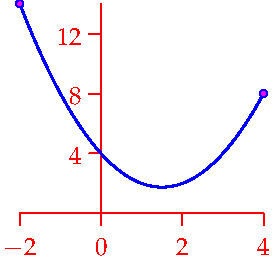
\includegraphics{unifcont3}\\
	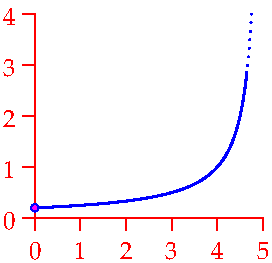
\includegraphics{unifcont4}
\end{examples}

\begin{proof}
	\begin{description}
		\item[\normalfont ($\Leftarrow$)] Suppose $g$ is well-defined; we leave the claim that it is continuous as an exercise, but by Theorem \ref{thm:unifclosed} it is uniformly so. Since $f=g$ on a subset $(a,b)\subseteq \dom g$, the same choice of $\delta$ will work for $f$ as it does for $g$: $f$ is therefore uniformly continuous.
		
		\item[\normalfont ($\Rightarrow$)] Suppose $f$ is uniformly continuous on $(a,b)$. Let $(x_n),(y_n)\subseteq (a,b)$ be sequences converging to $a$. To show that $g(a)$ is unambiguously defined, we must prove that $\bigl(f(x_n)\bigr)$ and $\bigl(f(y_n)\bigr)$ are convergent, and to the same limit.\par
		Define a sequence
		\[
			(u_n)=(x_1,y_1,x_2,y_2,x_3,y_3,\ldots)
		\]
		Plainly $\lim u_n=a$ since $(x_n)$ and $(y_n)$ have the same limit. But then $(u_n)$ is Cauchy; by Lemma \ref{lemm:unifcauchy}, $\bigl(f(u_n)\bigr)$ is also Cauchy and thus convergent. Since $\bigl(f(x_n)\bigr)$ and $\bigl(f(y_n)\bigr)$ are subsequences of a convergent sequence, they also converge to the same (finite!) limit.\par
		The case for $g(b)$ is similar.\qedhere
	\end{description}
\end{proof}


\goodbreak


\begin{examples}{}{funkysine}
	We finish with three related examples of continuous functions $f:\R\setminus\{0\}\to\R$; these will appear repeatedly as you continue to study analysis.
	\begin{enumerate}		
		\begin{minipage}[t]{0.6\linewidth}\vspace{0pt}
			\item $f(x)=\sin\frac 1x$ is continuous but \emph{not uniformly so.} To see this, note that $\textcolor{Green}{x_n=\frac 1{(n+\frac 12)\pi}}$ defines a Cauchy sequence ($\lim x_n=0$), and yet
			\[\textcolor{Magenta}{f(x_n)}=\sin\left(n+\frac 12\right)\pi=(-1)^n\]
			is not Cauchy since it diverges by oscillation.\par
			Consequently, there is no way to extend $f$ to a continuous function on any interval containing $x=0$.
		\end{minipage}
		\hfill
		\begin{minipage}[t]{0.39\linewidth}\vspace{0pt}
			\flushright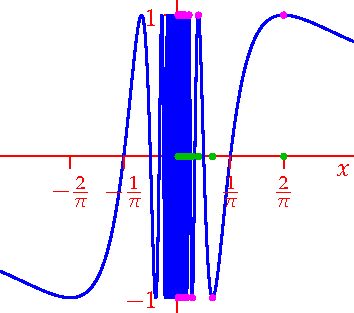
\includegraphics[scale=0.98]{unifcontex3}
		\end{minipage}\par
	  
	
		\begin{minipage}[t]{0.6\linewidth}\vspace{0pt}
			\item $f(x)=x\sin\frac 1x$ is \emph{uniformly continuous.} One way to see this is to extend the function to the origin by defining
			\[g(x)=\begin{cases}
			x\sin \frac 1x&\text{if }x\neq 0\\
			0&\text{if }x=0
			\end{cases}\]
			By the squeeze theorem, $\lim x_n=0\implies \lim f(x_n)=0$, so $g$ is well-defined and continuous on $\R$. By Theorem \ref{thm:unifext}, $f$ is uniformly continuous on any bounded interval. Moreover, the derivative
		\end{minipage}
		\hfill
		\begin{minipage}[t]{0.39\linewidth}\vspace{0pt}
			\flushright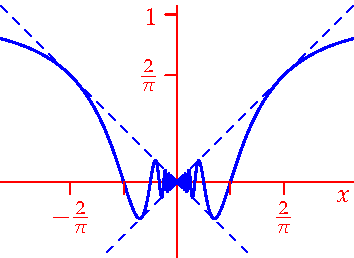
\includegraphics[scale=0.98]{unifcontex2}
		\end{minipage}\par\vspace{-4pt}
		\[
			f'(x)=\sin\frac 1x-\frac 1x\cos\frac 1x
		\]
		is bounded whenever $x$ is large; together with Exercise \ref{exs:unifcontunion} we could use this to conclude uniform continuity of $f(x)$. Note however that $f'(x)$ is unbounded when $x$ small ($\lim f'\left(\frac 1{2\pi n}\right)=\lim(-2\pi n)=-\infty$)
 so we can't use Theorem \ref{thm:unifbddderiv} to conclude that $f$ is uniformly continuous on its entire domain.

		\begin{minipage}[t]{0.6\linewidth}\vspace{-5pt}
			\item\label{ex:funkysine3} $f(x)=x^2\sin\frac 1x$ is also \emph{uniformly continuous}: again extend by $g(0)=0$. This time however, we could argue that the derivative is bounded
			\[
			\nm{f'(x)}=
				\nm{2x\sin\frac 1x-\cos\frac 1x}\le 3
			\]
			since $\nm{\sin y}\le\nm y$ for all $y$.\smallbreak
			
			In fact something stranger is going on. As you may verify (see Exercise \ref{exs:funkysine}), the \emph{extended function $g$ is everywhere differentiable} with $g'(0)=0$, and yet the derivative $g'(x)$ itself is \emph{discontinuous} at $x=0$!
% 			\[
% 				g'(0)=\lim_{x\to 0}\frac{g(x)-g(0)}x =\lim_{x\to 0}\frac 1x\sin\frac 1x=0
% 			\]
		\end{minipage}
		\hfill
		\begin{minipage}[t]{0.39\linewidth}\vspace{-5pt}
			\flushright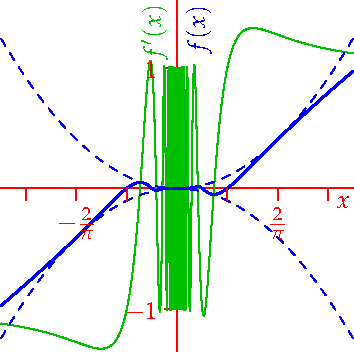
\includegraphics[scale=0.98]{unifcontex1}
		\end{minipage}
	\end{enumerate}
\end{examples}

\clearpage


\goodbreak


\begin{exercisessec}{}{}
	\exstart Decide whether each function is uniformly continuous on the given interval.
	Explain your answers.
	\begin{enumerate}\setcounter{enumi}{1}
	 	\item[]\begin{enumerate}
	 	  \item \makebox[180pt][l]{$f(x)=x^3$ on $[-2,4]$\hfill (b)} \ $f(x)=x^3$ on $(-2,4)$
	 	  \setcounter{enumii}{2}
	 	  \item \makebox[180pt][l]{$f(x)=x^{-3}$ on $(0,4]$\hfill (d)} \ $f(x)=x^{-3}$ on $(1,4]$
	 	  \setcounter{enumii}{4}
	 	  \item \makebox[180pt][l]{$f(x)=e^x$ on $(-\infty,100)$\hfill (f)} \ $f(x)=e^x$ on $\R$
	 	\end{enumerate}
	 	 
  \item%[2.]modified
   Prove that each function is uniformly continuous on the indicated domain by verifying the $\epsilon$-$\delta$ property.
   \begin{enumerate}
	  \item \makebox[180pt][l]{$f(x)=3x+11$ on $\R$ \hfill (b)} \ $f(x)=x^2$ on $[0,3]$
	  \setcounter{enumii}{2}
	  \item \makebox[180pt][l]{$f(x)=\frac 1{x^2}$ on $[\frac 12,\infty)$\hfill (d)} \ $f(x)=\frac{x+2}{x+1}$ on $[0,1]$
  \end{enumerate}
  
  \item\label{exs:funkysine} Verify the claim in Example \ref*{ex:funkysine}.\ref{ex:funkysine3} that the function $g(x)$ is differentiable at zero\footnotemark{} but that the derivative $g'(x)$ is discontinuous there.
  
  \item%[4.]
  \begin{enumerate}
  	\item If $f$ is uniformly continuous on a bounded set $U$, prove that $f$ is bounded on $U$.\par
  	(\emph{Hint: for contradiction, assume $\exists (x_n)\subseteq U$ for which $\nm{f(x_n)}\to\infty\ldots$})
  	\item Use (a) to give another proof that $\frac 1{x^2}$ is not uniformly continuous on $(0,1)$.
  	\item Give an example to show that a uniformly continuous function on an \emph{unbounded} set $U$ could be unbounded.
  \end{enumerate}
  
  
  
%   \item[6.]\begin{enumerate}
%   \item Let $f(x)=\sqrt x$ for $x\ge 0$. Show that $f'$ is unbounded on $(0,1]$, but that $f$ is nevertheless uniformly continuous on $(0,1]$.
%   \item Show that $f$ is uniformly continuous on $[1,\infty)$.
%   \end{enumerate}
  
%   \item%[8.]
%   \begin{enumerate}
%   	\item Use the Mean Value Theorem to prove that
%   	\[\nm{\sin x-\sin y}\le \nm{x-y}\]
%   	for all $x,y\in\R$.
%   	\item Show that $\sin x$ is uniformly continuous on $\R$.
%   \end{enumerate}
  
%   \item[10.] Let $f(x)=x^2\sin(\frac 1x)$ for $x\neq 0$ and $f(0)=0$
%   \begin{enumerate}
%   \item Observe that $f$ is continuous on $\R$.
%   \item Why is $f$ uniformly continuous on any bounded subset of $\R$?
%   \item Is $f$ uniformly continuous on $\R$?
%   \end{enumerate}
  
  % 	\begin{enumerate}
% 	  \item If $0<a<b\le\infty$, then $f:(a,b)\to\R:x\mapsto\frac 1{x^3}$ is uniformly continuous.\\[5pt]
% 	  Let $\epsilon>0$ be given and let $\delta=\frac 13a^4\epsilon$. Then, $\forall x,y\in(a,b)$,
% 	  \begin{align*}
% 	  	\nm{x-y}<\delta\implies \nm{f(x)-f(y)}&=\nm{\frac 1{x^3}-\frac 1{y^3}}=\frac{\nm{y^3-x^3}}{x^3y^3}=\frac{(x^2+xy+y^2)\nm{x-y}}{x^3y^3}\\
% 	  	&<\left(\frac 1{xy^3}+\frac 1{x^2y^2}+\frac 1{x^3y}\right)\delta <\frac 3{a^4}\delta=\epsilon
% 	  \end{align*}
% 	  
% 	  \item If $0<b\le\infty$, then $f:(0,b)\to\R:x\mapsto\frac 1{x^3}$ is not uniformly continuous.\\[5pt]
% 	  Let $\epsilon=1$ and let $\delta>0$ be given. Let $x=\min\{1,\delta\}$ and $y=\min\{\frac 12,\frac\delta 2\}$. Then
% 	  \[\nm{x-y}=\begin{cases}
% 	  \frac 12&\text{if }\delta\ge 1\\
% 	  \frac\delta 2&\text{if }\delta<1
% 	  \end{cases}\]
% 	  Certainly $\nm{x-y}<\delta$. However,
% 	  \[\nm{f(x)-f(y)}=\nm{\frac 1{x^3}-\frac 1{y^3}}=\begin{cases}
% 	  \nm{1-8}=7&\text{if }\delta\ge 1\\
% 	  \nm{\delta^{-3}-8\delta^{-3}}=7\delta^{-3}&\text{if }\delta<1
% 	  \end{cases}\]
% 	  In either case, $\nm{f(x)-f(y)}\ge 7>1=\epsilon$, whence $f$ is not uniformly continuous.
% 	\end{enumerate}


		\item Suppose $g$ is defined on $U$ and $a\in U$. Give \emph{very brief} (one line!) arguments for the following.
		\begin{enumerate}
		  \item Prove that $g$ is continuous at $a$ provided
		  \[\forall \epsilon>0,\ \exists \delta>0\text{ such that }0<\nm{x-a}<\delta\implies\nm{g(x)-g(a)}<\epsilon\]
		  %This is trivial, since $x=a$ automatically makes the RHS zero.
		  \item Prove that $g$ is continuous at $a$ provided
		  \[\forall (x_n)\subseteq U\setminus\{a\},\ \lim x_n=a\implies \lim g(x_n)=g(a)\]
		  %Apply the argument in Theorem \ref{thm:cont} to part (a).
		  \item Verify that the function $g$ defined in Theorem \ref{thm:unifext} is indeed continuous whenever it is well-defined.
		  %By definition, $g(a)=\lim f(x_n)=\lim g(x_n)$ whenever $(x_n)\subseteq U\setminus\{a\}$, etc.
		\end{enumerate}


  \item\label{exs:unifcontunion}\begin{enumerate}
    \item Suppose $f$ is uniformly continuous on intervals $U_1,U_2$ for which $U_1\cap U_2$ is non-empty. Prove that $f$ is uniformly continuous on $U_1\cup U_2$.\par
    (\emph{Hint: if $x,y$ do not lie in the same interval $U_i$, choose some $a\in U_1\cap U_2$ between $x$ and $y$})

		\item Prove that $f(x)=\sqrt x$ is uniformly continuous on $[0,\infty)$.
		
		\item More generally, prove that any root function $f(x)=x^{1/n}$ ($n\in\N$) is uniformly continuous on its domain ($\R$ if $n$ is odd and $[0,\infty)$ if $n$ is even).
		
		\item (Hard) \ Given $f(x)=x^{1/n}$, show that $\delta=\epsilon^n$ demonstrates uniform continuity when $n$ is even and $\delta=\left(\frac\epsilon 2\right)^n$ when $n$ is odd.\par
		(\emph{Hint: use the binomial theorem to prove that $0\le y<x+\delta\implies y^{1/n}<x^{1/n}+\delta^{1/n}$})
% 	 Indeed if $\epsilon>0$ is given and $\delta=\epsilon^n$, then\footnote{WLOG $x\ge y\ge 0$. Then
% 	\begin{align*}
% 	\nm{x-y}<\delta&\implies 0\le x<y+\delta\implies x^{1/n}<y^{1/n}+\delta^{1/n}\tag*{(by the binomial theorem)}\\
% 	&\implies 0\le x^{1/n}-y^{1/n}<\delta^{1/n}=\epsilon
% 	\end{align*}}
% 	\[\forall x,y\ge 0,\ \nm{x-y}<\epsilon^n\implies \nm{x^{1/n}-y^{1/n}}<\epsilon\]
% 	Odd roots are also uniformly continuous, but on the whole domain $\R$: when $n$ is odd $\delta=\left(\frac\epsilon 2\right)^n$ does the job,\footnote{If $x\ge y\ge 0$ we're done by the above, since $\left(\frac\epsilon 2\right)^n<\epsilon^n$. If $x\le y\le 0$, replace $X=-x$ and $Y=-y$ to see that we're again done. Finally, if $x\ge 0\ge y$, then $x<\delta+y<\delta$ and $-y<\delta-x<\delta$. But then
% 	  \[0<x^{1/n}-y^{1/n}<2\delta^{1/n}=\epsilon\]}
% 	\[\forall x,y\in\R,\ \nm{x-y}<\left(\frac\epsilon 2\right)^n\implies \nm{x^{1/n}-y^{1/n}}<\epsilon\]
	\end{enumerate}

\end{enumerate}
\end{exercisessec}

\vspace{-15pt}

\footnotetext{Use the definition $g'(0)=\lim\limits_{x\to 0}\frac{g(x)-g(0)}{x-0}$. Limits of functions are covered formally in the next section (course!), but you should be familiar with the idea from elementary calculus.}